%%%%%%%%%%%%%%%%%%%%%%%Preamble%%%%%%%%%%%%%%%%%%%%%%%%%%%
\documentclass[11pt]{article}
\usepackage[a4paper,margin=1in]{geometry}
\usepackage{fontspec}
\setmainfont{Arial}
\usepackage{graphicx}
\usepackage[table]{xcolor}
\usepackage{array}
\usepackage{setspace}
\onehalfspacing
\usepackage{booktabs}
\usepackage{multirow}
\usepackage{parskip}   
\usepackage{amsmath}
\usepackage{amssymb}
\usepackage{microtype}
\usepackage{lipsum}  
\usepackage{etoolbox}
\usepackage{cite}
\usepackage{tocloft}
\renewcommand{\cftsecnumwidth}{2cm}
\renewcommand{\cftsecaftersnum}{: }
\renewcommand{\cftsecpagefont}{\normalfont\bfseries}
\renewcommand{\cftsecpresnum}{Chapter\ }
\usepackage{caption}
\usepackage{ifthen}
\usepackage{float}
\usepackage[intoc]{nomencl}
\makenomenclature
\usepackage{titlesec}
\usepackage{chngcntr}
\titleformat{\section}
  {\centering\normalfont\Large\bfseries}
  {Chapter \thesection :}{1em}{}
\patchcmd{\listoffigures}{\section*{\listfigurename}}{\section*{\centering \listfigurename}}{}{}
\patchcmd{\listoftables}{\section*{\listtablename}}{\section*{\centering \listtablename}}{}{}
\renewcommand{\cftdotsep}{1.5}
\renewcommand{\cftsecleader}{\cftdotfill{\cftdotsep}}
\renewcommand{\cftfigleader}{\cftdotfill{\cftdotsep}}
\renewcommand{\cfttableader}{\cftdotfill{\cftdotsep}}
\renewcommand{\contentsname}{Table of Contents}
\renewcommand{\nomname}{\centering List of Symbols}
\renewcommand{\cftfigpresnum}{Figure~}
\renewcommand{\cftfigaftersnum}{\hspace{0.5em}}
\renewcommand{\cfttabpresnum}{Table~}
\renewcommand{\cfttabaftersnum}{\hspace{0.5em}} 
\settowidth{\cftfignumwidth}{Figure 10\quad}
\settowidth{\cfttabnumwidth}{Table 10\quad}
\renewcommand{\cfttoctitlefont}{\hfill\Large\bfseries}
\renewcommand{\cftaftertoctitle}{\hfill\textnormal{\textbf{Page}}}
\renewcommand{\cftloftitlefont}{\hfill\Large\bfseries}
\renewcommand{\cftafterloftitle}{\hfill\textnormal{\textbf{Page}}}
\renewcommand{\cftlottitlefont}{\hfill\Large\bfseries}
\renewcommand{\cftafterlottitle}{\hfill\textnormal{\textbf{Page}}}
\captionsetup[figure]{labelsep=period}
\captionsetup[table]{labelsep=period}
\usepackage[hidelinks]{hyperref}
% Let long URLs (e.g. the NeurIPS proceedings hash links in the bibliography)
% stretch and break across lines instead of producing underfull/overfull boxes.
% \UrlOrds permits breaks at ordinary characters, so a long hash breaks cleanly.
\Urlmuskip=0mu plus 3mu\relax
\makeatletter
\g@addto@macro{\UrlBreaks}{\UrlOrds}
\makeatother
%%%%%%%%%%%%%%%%%%%%%%%%%%%Document Start%%%%%%%%%%%%%%%%%

\begin{document}


% ---------- Title Page ----------
\begin{titlepage}
\begingroup
\setmainfont{Times New Roman}
\fontsize{16}{19}\selectfont
\begin{flushright}
  
\includegraphics[width=0.4\textwidth]{Figures/kcl.png}
\end{flushright}

\vspace*{1cm}

\begin{center}
    {\textbf{King’s College London}}\\[1.5cm]
    {\fontsize{18}{21}\selectfont \textbf{CAPIM: Confidence-Aware PIM-based Architecture for LLM Inference on Mobile Devices}}\\[1cm]
    {\textbf{Submitted by:}}\\[0.1cm]
    {\textbf{Idan Hochman}}\\[0.1cm]
    {\textbf{k25107212}}\\[1cm]
    {\textbf{Project Report Submitted in Partial Fulfillment of the Requirements of the MSc Project Module}}\\[1cm]
    {\textbf{Engineering Department}}\\[1cm]
    {\textbf{Supervised by:}}\\[0.3cm]
    {\textbf{Dr. Haiyu Mao}}\\[1.5cm]
    {\textbf{London}}\\[0.2cm]
    {\textbf{August 2026}}
\end{center}
\endgroup
\end{titlepage}
\pagenumbering{roman}


% ---------- Declaration Section ----------

\newpage
\section*{\centering Declaration}

I declare that parts of this submission have contributions from AI software and that it aligns with acceptable use as specified as part of the assignment brief/ guidance and is consistent with good academic practice. The content can still be considered as my own words. I understand that as long as my use falls within the scope of appropriate use as defined in the assessment brief/guidance then this declaration will not have any direct impact on the grades awarded.

I acknowledge use of software to:
\begin{itemize}
    \item Generate ideas or structure suggestions, for assistance with understanding core concepts, or other substantial foundational and preparatory activity:
    \begin{itemize}
        \item Gemini
        \item NotebookLM
        \item Claude
    \end{itemize}
    \item Write, rewrite, rephrase and/or paraphrase part of this essay:
    \begin{itemize}
        \item Claude
    \end{itemize}
\end{itemize}


% ---------- Abstract Section ----------

\newpage
\section*{\centering Abstract}
\addcontentsline{toc}{section}{Abstract}

On-device LLM inference offers privacy and latency benefits, but mobile platforms have only a fraction of a data centre's memory bandwidth and energy budget, and generating each token requires streaming the model's full weights from memory. Processing-in-memory (PIM) cuts this movement cost; speculative decoding supplies the parallelism a device serving one request at a time cannot get from batching. LP-Spec, a state-of-the-art mobile PIM architecture, adopts Medusa speculative decoding, drafting candidate token trees and pruning them using retrospective, content-blind acceptance statistics to save energy during verification.

This project asks whether a mobile PIM architecture can instead exploit EAGLE-2, a speculative decoding method that computes a live, per-token confidence score for each drafted token. It asks whether such an architecture can replace Medusa drafting and outperform LP-Spec, and whether EAGLE-2's confidence scores, currently used only to rank candidate branches, can instead gate a branch's expansion directly.

The project proposes CAPIM, which integrates EAGLE-2 natively. A confidence gate stops each draft branch once its accumulated log-probability falls below a threshold, and the resulting tree size selects, against a second threshold, whether verification stays PIM-resident or splits with the NPU. CAPIM is evaluated by analytical simulation on Vicuna-7B-v1.3 over Alpaca and GSM8K datasets, priced on one cost model against LP-Spec and autoregressive decoding.

CAPIM reaches 1.45×--2.00× LP-Spec's best simulated energy efficiency and 1.09×--1.21× its throughput. These results validate confidence-gated pruning and run-time verification routing as an effective basis for energy-efficient, low-latency on-device LLM inference. The architecture also lets the device control the energy--latency trade-off directly, setting the routing threshold to match its own battery and thermal state.


% ---------- Table of Contents ----------

\newpage
\begin{spacing}{1.5}
  \addcontentsline{toc}{section}{Table of Contents}
  \tableofcontents
\end{spacing}



% ---------- List of Tables ----------
\newpage
\section*{\centering \normalsize \listoftables}
\addcontentsline{toc}{section}{List of Tables}


% ---------- List of Figures ----------
\newpage
\section*{\centering\normalsize\listoffigures}
\addcontentsline{toc}{section}{List of Figures}

% ---------- List of Symbols ----------
\newpage

% Group headings for the List of Symbols (Acronyms then Notation)
\renewcommand{\nomgroup}[1]{%
  \ifthenelse{\equal{#1}{A}}{\item[\textbf{Acronyms}]}{%
  \ifthenelse{\equal{#1}{B}}{\bigskip\item[\textbf{Notation}]}{}}%
}

% ---- Acronyms ----
\nomenclature[a-ALU]{ALU}{Arithmetic Logic Unit}
\nomenclature[a-CPU]{CPU}{Central Processing Unit}
\nomenclature[a-DMA]{DMA}{Direct Memory Access}
\nomenclature[a-DRAM]{DRAM}{Dynamic Random Access Memory}
\nomenclature[a-EDP]{EDP}{Energy-Delay Product}
\nomenclature[a-FC]{FC}{Fully-Connected}
\nomenclature[a-GEMM]{GEMM}{General Matrix Multiplication}
\nomenclature[a-GPU]{GPU}{Graphics Processing Unit}
\nomenclature[a-HBM]{HBM}{High Bandwidth Memory}
\nomenclature[a-LLM]{LLM}{Large Language Model}
\nomenclature[a-LPDDR]{LPDDR}{Low-power Double Data Rate}
\nomenclature[a-MAC]{MAC}{Multiply-Accumulate}
\nomenclature[a-NPU]{NPU}{Neural Processing Unit}
\nomenclature[a-PIM]{PIM}{Processing-in-Memory}
\nomenclature[a-PNM]{PNM}{Processing-Near-Memory}
\nomenclature[a-PUM]{PUM}{Processing-Using-Memory}
\nomenclature[a-QKV]{QKV}{Query, Key and Value}
\nomenclature[a-SIMD]{SIMD}{Single Instruction, Multiple Data}
\nomenclature[a-SRAM]{SRAM}{Static Random Access Memory}

% ---- Notation ----
% Each symbol is written exactly as the body renders it: text mode where the body
% uses text mode, math mode where the body uses math mode.
\nomenclature[b-01]{σ\textsubscript{th}}{Model confidence score threshold}
\nomenclature[b-02]{μ}{Draft tree size, in surviving nodes}
\nomenclature[b-03]{μ\textsubscript{th}}{Candidate token tree size threshold}
\nomenclature[b-04]{L\textsubscript{spec}}{LP-Spec's speculation length, in retained candidate tokens}
\nomenclature[b-05]{$t_{\text{layer}}$}{Latency of a typed layer}
\nomenclature[b-06]{$c_{\text{layer}}$}{Operation count of a typed layer}
\nomenclature[b-07]{$b_{\text{layer}}$}{Bytes a typed layer must move}
\nomenclature[b-08]{$\Pi_{\text{device}}$}{Peak compute throughput of a device}
\nomenclature[b-09]{$B_{\text{device}}$}{Relevant bandwidth of a device}
\nomenclature[b-10]{$N_{\text{ALU}}$}{Near-bank ALUs per PIM compute unit, and hence nodes verified per pass}
\nomenclature[b-11]{$t_n$}{Time the NPU alone would take on an undivided kernel}
\nomenclature[b-12]{$t_p$}{Time PIM alone would take on an undivided kernel}
\nomenclature[b-13]{$r$}{Fraction of a kernel's output columns routed to the NPU}
\nomenclature[b-14]{$t_{\text{kernel}}$}{Makespan of a column-split kernel}
\nomenclature[b-15]{$K$}{Number of tokens generated during decoding}

\printnomenclature

%%%%%%%%%%%%%%%%%%%%%%%%%%%%%%%%%%%%%%%%%%%%%%%%%%%%%%%%%%%%%%

% ---------- Acknowledgements ----------
\newpage
\section*{\centering Acknowledgements}
\addcontentsline{toc}{section}{Acknowledgements}

I would like to thank Dr. Haiyu Mao for supervising this project. Her guidance and feedback throughout shaped both the direction of the research and the rigour with which it was carried out.

% ---------- Main body starts here ----------
\newpage
\pagenumbering{arabic}
\setcounter{page}{1}


% ---------- Introduction ----------
\section{Introduction}

\subsection{Background}
Large Language Models (LLMs) have become highly successful and widely adopted, yet they are still run predominantly in the cloud, with mobile and edge devices acting as thin clients that send each request to a remote server. Performing inference on the device itself would instead keep user data local, remove the network delay and jitter of a cloud round-trip, and preserve service availability without a connection. These benefits are difficult to attain in practice, because a mobile platform offers only a fraction of the memory bandwidth, compute, and energy of a data-centre server. Delivering on-device inference within those limits calls for new architectural approaches rather than scaled-down server designs.

The binding constraint is not the arithmetic but the movement of data. To generate a token, the model must stream its full set of weights out of memory, and in a conventional processor-centric system it is this movement across the off-chip interface, rather than the computation performed once the data arrives, that dominates both energy and latency. The imbalance is most severe at the edge: when large neural-network models run on modern edge accelerators, more than 90\% of the total system energy is spent on memory rather than on computation~\cite{mutlu2022primer}. On a device drawing from a fixed battery, energy efficiency is therefore the primary objective, and reducing data movement is the most direct means of improving it.

Processing-in-Memory (PIM) attacks this bottleneck at its source. It is a data-centric paradigm that places compute units directly inside or near the memory arrays, so that the weights are processed where they already reside instead of being moved to a central processor across an external bus~\cite{mutlu2022primer}. By removing that movement, it directly attacks the cost that dominates energy on a battery-constrained device.

Speculative decoding addresses a second and complementary constraint: the latency of the sequential decoding stage. An LLM generates its output one token at a time, each conditioned on all tokens before it, so decoding is inherently serial. Parallelism can be achieved by batching many independent user requests and decoding them together, but this requires a supply of concurrent requests; an on-device system serves a single user stream and is restricted to a batch size of one. Speculative decoding instead extracts parallelism from that single stream by cheaply drafting several candidate tokens and verifying them together in one pass~\cite{leviathan2023speculative}, making it the primary means of accelerating decoding on the device.

A PIM-based architecture that accelerates decoding with speculative decoding therefore addresses both constraints at once, and is a natural direction for efficient on-device inference. Prior work has pursued it: LP-Spec~\cite{he2025lpspec} is among the current state-of-the-art mobile PIM architectures, running speculative decoding on an LPDDR5-PIM substrate and scheduling the verification work between the PIM units and a mobile NPU. It is the baseline this work builds upon.

\subsection{Problem statement}
LP-Spec~\cite{he2025lpspec}, a state-of-the-art mobile PIM architecture, uses Medusa for speculative decoding. Medusa attaches extra decode heads to the model, which emit a static candidate tree in a single parallel pass~\cite{cai2024medusa}. Generating the branches is therefore cheap, and the cost lies in verifying them, which grows with the size of the tree. To bound that cost, LP-Spec prunes the tree as it is built, keeping the branches most likely to be accepted. The branches it keeps, however, are chosen from retrospective statistics -- aggregate acceptance rates per head and tree position, accumulated over past decoding iterations. The pruning is thus content-blind: two different contexts at the same tree position are handed much the same tree, regardless of what the model actually predicts for the text being generated now.

More recent speculative decoding methods outperform Medusa, and EAGLE-2 is among the strongest of them. It drafts autoregressively at the feature level, and for each proposed token it produces a live confidence score, with higher scores tending to correspond to a greater chance that the token is accepted in the current context~\cite{li2024eagle2}. EAGLE-2 already uses these scores to shape its draft tree, but only to rank branches for expansion; the tree still grows to a fixed size whether the context is confident or uncertain. Because they are computed for the current context rather than accumulated from history, these scores might serve as a more accurate pruning criterion than LP-Spec's retrospective one. Yet, to the best of our knowledge, no mobile PIM architecture has adopted EAGLE-2 or used its confidence scores to prune the draft tree and spare the energy of verifying branches unlikely to be accepted.

Pruning is not the only decision such an architecture makes at run-time; it must also route the verification work between the PIM units and the NPU. LP-Spec's Data Allocation Unit always offloads a share of that work to the NPU to minimize latency, so a portion of the weights crosses the off-chip interface on every iteration -- the dominant energy cost -- with no way to prefer the slower but cheaper in-memory placement when the battery is low. The size of a confidence-shaped draft tree could instead inform this choice, trading energy against latency according to the device's battery and thermal state.

\subsection{Proposed solution}
This project proposes CAPIM, a confidence-aware PIM-based architecture for LLM inference on mobile devices that natively integrates EAGLE-2. Its central mechanism is a confidence gate: during drafting, the architecture tracks each branch's accumulated confidence and terminates the branch once that confidence falls below a configurable threshold. This gate is CAPIM's pruning stage, replacing LP-Spec's retrospective pruner with one driven by the live confidence signal. Because a branch is stopped as soon as its confidence runs out, the size of the tree follows the context -- large when the model is confident, small when it is uncertain.

The size of the pruned tree in turn informs where verification runs, between the PIM units and the NPU, against a second threshold. This threshold is not a fixed, latency-driven split but a run-time control the device can set according to its battery and thermal state. When the tree is small, verification stays resident in the PIM units and avoids the off-chip weight traffic that dominates energy; a higher-performance setting instead splits the work onto the NPU for speed. The energy-latency trade-off is thereby exposed as a run-time choice, rather than fixed to latency as in LP-Spec's Data Allocation Unit.

CAPIM is evaluated by architectural simulation against LP-Spec and a plain autoregressive baseline, all priced on a shared cost model so that any difference reflects the designs and not how they were measured. CAPIM improves energy efficiency over the LP-Spec baseline while also improving latency, with the full results presented in Chapter 5.

\subsection{Report outline}
The rest of this report is organized as follows. Chapter 2 reviews the relevant literature on PIM, PIM-based inference architectures, and speculative decoding. Chapter 3 defines the research problem, the research questions, and the project objectives. Chapter 4 presents the methodology, covering both the proposed CAPIM architecture and the simulation framework used to evaluate it. Chapter 5 reports the results, from the characterization of EAGLE-2's draft trees under a confidence gate through to the headline comparison against the baselines. Finally, Chapter 6 concludes the report and discusses directions for future work.

% ---------- Chapter Two ----------
\newpage
\section{Literature Review}

\subsection{Processing-in-memory (PIM)}
PIM is a data-centric computing paradigm designed to overcome the performance and energy bottlenecks of traditional processor-centric systems. The core principle of PIM is placing computation mechanisms directly inside or near where data is stored, rather than moving data to a central processor, like traditional computer architectures. Data movement is a key bottleneck for data-intensive domains, such as machine learning and genome analysis, in terms of energy and latency costs. PIM architectures aim to mitigate those costs by eliminating the need for data movement~\cite{mutlu2022primer}.

This bottleneck is structural and worsening. Conventional systems are processor-centric: they are designed to move data to computation, yet the cost of moving data, especially between off-chip memory and the on-chip processor, far exceeds the cost of the computation itself in terms of energy, latency and bandwidth. The imbalance is a direct consequence of technology scaling. Between 1999 and 2017, DRAM capacity improved by roughly 128×, but memory bandwidth improved by only about 20×, while memory latency remained nearly constant, improving by only around 30\% over two decades~\cite{mutlu2022primer}. The resulting ``memory wall'' is especially punishing for mobile and edge workloads, where data movement dominates the energy budget. For widely-used mobile consumer workloads, more than 62\% of the total system energy of a mobile device is spent on data movement between the processor and the memory hierarchy, and for large commercial edge neural-network models running on modern edge accelerators, more than 90\% of the system energy is consumed by memory~\cite{mutlu2022primer}. On-device LLM inference is an even more memory-intensive instance of this same problem, as it is dominated by a sequential, memory-bound decoding stage. This makes reducing data movement, rather than accelerating computation, the primary lever for energy efficiency in battery-constrained deployment.

PIM designs fall into two broad categories. Processing-Using-Memory (PUM) exploits the analog operational principles of the memory circuitry itself to perform massively parallel operations in situ, such as bulk copy, bitwise Boolean logic and simple arithmetic within the memory arrays. Processing-Near-Memory (PNM) instead adds explicit compute logic, such as accelerators, simple cores or reconfigurable units, close to the memory arrays, for example in the logic layer of a 3D-stacked device or near individual DRAM banks. PNM provides high-bandwidth, low-energy and low-latency access to data while retaining a conventional programmable compute model~\cite{mutlu2022primer}. The architectures relevant to this project, including PAPI and LP-Spec (discussed below) as well as the proposed CAPIM, are all PNM designs.

\subsection{LLM inference}
Modern LLMs are built from a stack of transformer decoder blocks. Each block comprises four principal kernels: QKV (query, key, and value) generation, multi-head attention, projection, and a feedforward network. Text is generated autoregressively: the model emits one token at a time, and each new token is conditioned on the entire sequence produced so far. To avoid recomputing the attention keys and values for the whole sequence at every iteration, the K and V matrices are cached once produced and reused across all subsequent iterations, a mechanism known as the KV-cache~\cite{he2025papi}.

Inference divides into two stages. In the \emph{prefill} stage, the model processes all tokens of the input prompt simultaneously to produce the first output token; this is a highly parallel, compute-bound operation. In the \emph{decoding} stage, the model runs many sequential iterations, each taking the previously generated token as input to produce the next one, so generating $K$ output tokens requires $K$ dependent iterations. The decoding stage dominates end-to-end latency: for the GPT-3 175B model with input and output lengths of 32, serial decoding accounts for roughly 96\% of the total execution time~\cite{he2025papi}. This makes decoding the primary target for optimization. The two stages are illustrated in Figure~\ref{fig:llm_inference}.

Because decoding is inherently sequential, producing only a single token per iteration, it is the natural target for efficiency improvements. Two parallelism techniques are commonly employed to accelerate it. The first is \emph{batching}, in which several independent user requests are grouped and processed together in one pass; the number of sequences handled simultaneously is termed the \emph{batch size}. Because the model weights loaded for one iteration are shared across every request in the batch, batching amortizes the cost of decoding over many tokens at once. The second is \emph{speculative decoding}, in which several candidate tokens are proposed and verified together within a single decoding iteration instead of one at a time (discussed in detail in Section~\ref{subsec:sd}). Both techniques raise the number of tokens processed per decoding iteration, and thereby improve efficiency.

\begin{figure}[H]
\centering
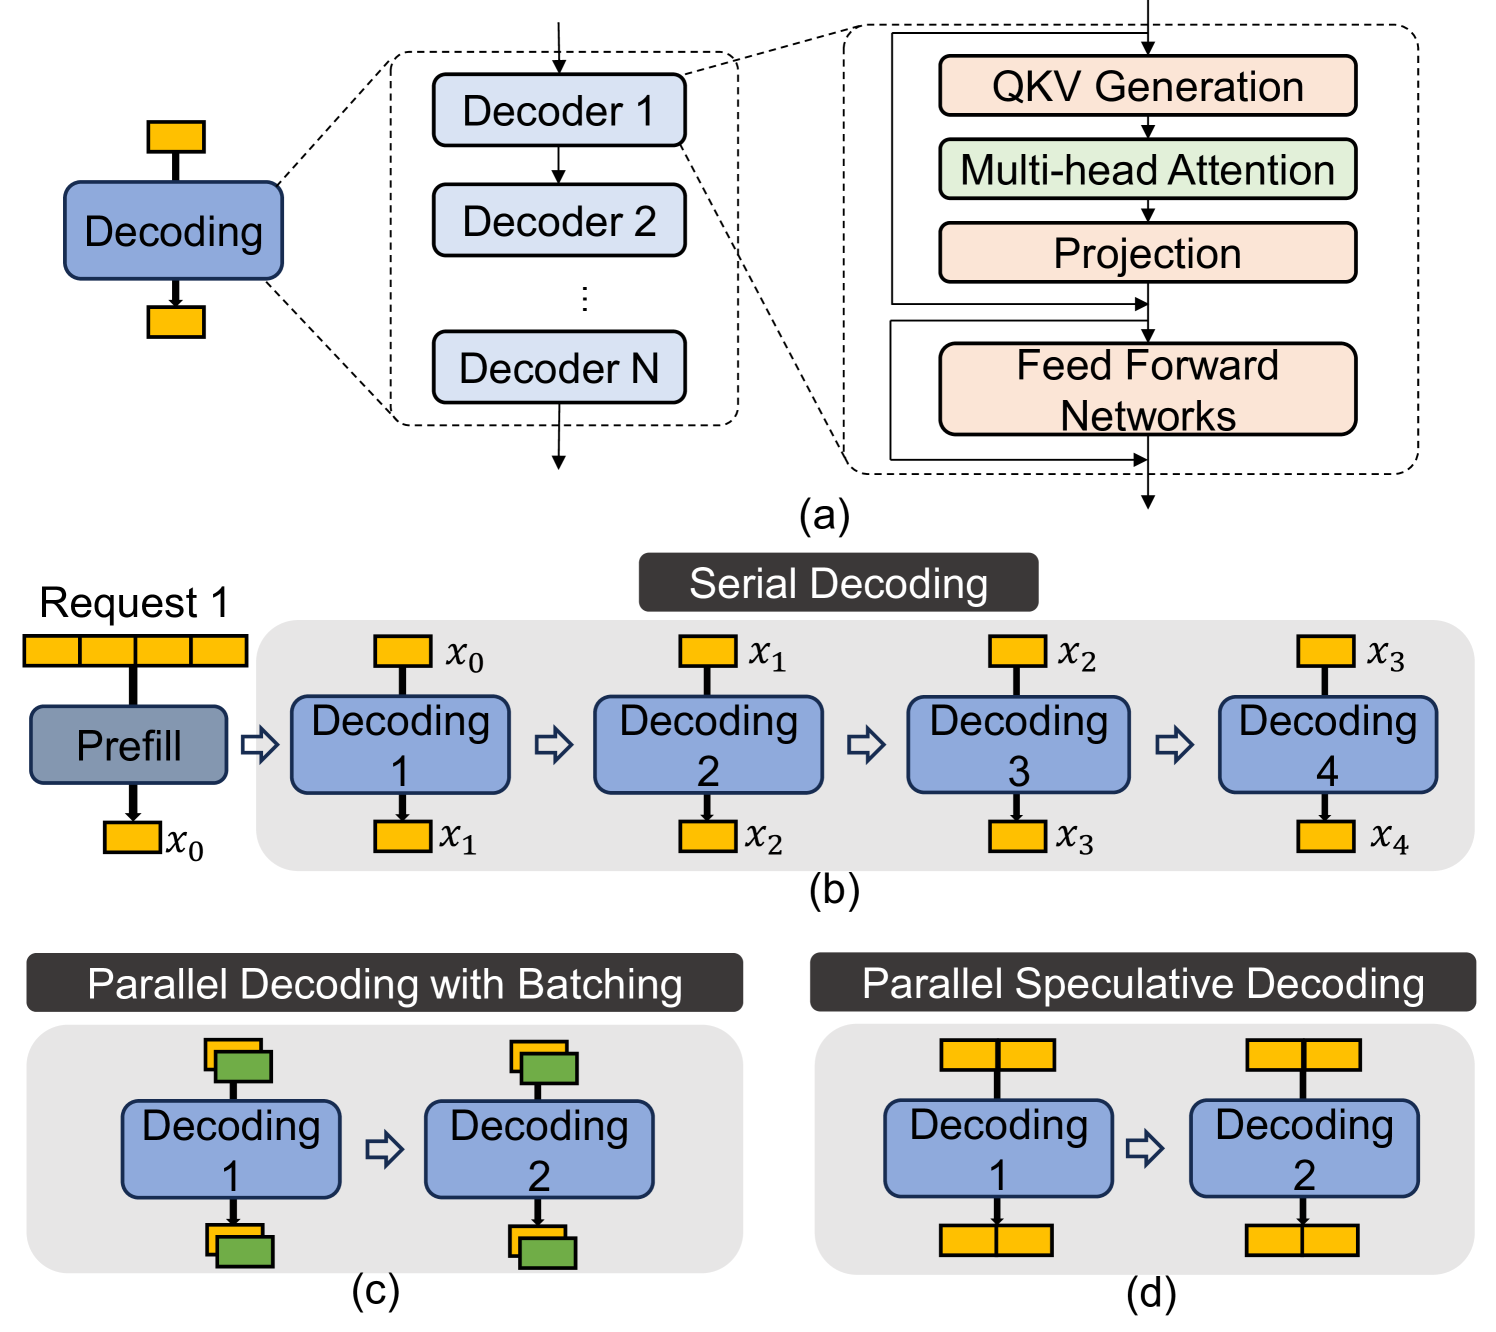
\includegraphics[width=0.75\textwidth]{Figures/papi_figure1_llm_inference.png}
\caption[LLM inference: prefill and decoding stages]{LLM inference: prefill and decoding stages (reproduced from~\cite{he2025papi}).}
\label{fig:llm_inference}
\end{figure}

\subsection{PAPI: PIM-based LLM inference architecture}\label{subsec:papi}
A central insight for accelerating decoding on PIM-based architectures is that whether a given decoding kernel is compute-bound or memory-bound is not a fixed property, but depends on how much parallelism is available. This distinction is only actionable on a heterogeneous platform that pairs a conventional processor with PIM, where each kernel can be steered to the resource that suits it; a system built around a single compute unit, such as a GPU alone, cannot exploit it. The parallelism in question has two sources: the batch size, which sets the number of requests processed together, and the speculative decoding length, which sets the number of candidate tokens evaluated per decoding iteration. A kernel's arithmetic intensity, defined as the number of floating-point operations it performs per byte of data accessed from memory, grows with the product of these two quantities, so the same kernel can sit on either side of the roofline depending on the operating point~\cite{he2025papi}.

This yields a concrete characterization of the decoding kernels. The fully-connected (FC) kernels (QKV generation, projection, and the feedforward network) are compute-bound when the available parallelism, and hence their arithmetic intensity, is large, and memory-bound otherwise. The attention kernel, by contrast, is always memory-bound, regardless of the available parallelism. It is therefore the FC kernels alone whose classification shifts with the operating point~\cite{he2025papi}.

Parallel Decoding with PIM (PAPI) is built directly on this characterization. It classifies each kernel at runtime from the batch size and speculative decoding length, dispatching compute-bound kernels to a conventional processing unit and memory-bound kernels to PIM modules, so that each kernel runs on the hardware best suited to it~\cite{he2025papi}. PAPI is, however, a server-class architecture rather than a mobile one: driving the FC kernels into the compute-bound regime depends on batching many concurrent user requests, an assumption that does not hold for on-device inference, where requests arrive one at a time. Carrying this compute-versus-memory-bound scheduling insight into the mobile setting is the subject of the architectures discussed below.

\subsection{Speculative decoding techniques}\label{subsec:sd}
Speculative decoding was developed to mitigate the inefficiencies of LLM inference. Because autoregressive decoding is inherently serial (producing one token at a time), improving performance required introducing more parallelism.

Traditional speculative decoding (speculative sampling) achieved this by using a smaller, separate draft model to quickly propose a sequence of tokens, which the larger target model then verifies in parallel~\cite{leviathan2023speculative}. Verification accepts each proposed token with a probability set by how the target model's own probability for it compares to the draft model's. A rejected token is not simply dropped: a replacement is resampled from a distribution corrected for what the draft got wrong, so the sequence that results follows exactly the same distribution as sampling from the target model alone would. This is what makes speculative decoding lossless, and the guarantee holds for any draft model, regardless of its quality~\cite{leviathan2023speculative}. The draft therefore governs only how many tokens are accepted per iteration, and hence the achieved speedup, never the correctness of the output. A direct consequence, which the pruning mechanism proposed in this work relies upon, is that discarding a draft token, even one that would eventually have been accepted, can only cost speed; it can never alter the generated text.

Next-generation speculative decoding techniques introduced tree-based generation, verifying multiple candidates simultaneously. One of those techniques is Medusa. Medusa attaches multiple extra decoding heads directly to the final layer of the model. These heads allow the model to predict the next token, the token after that, and so on, all from a single hidden state, eliminating the need for a separate draft model~\cite{cai2024medusa}. The predictions of these heads are assembled into a static candidate tree, whose structure is fixed in advance and processed in parallel using tree-based attention. The Medusa workflow is shown in Figure~\ref{fig:medusa}.

\begin{figure}[H]
\centering
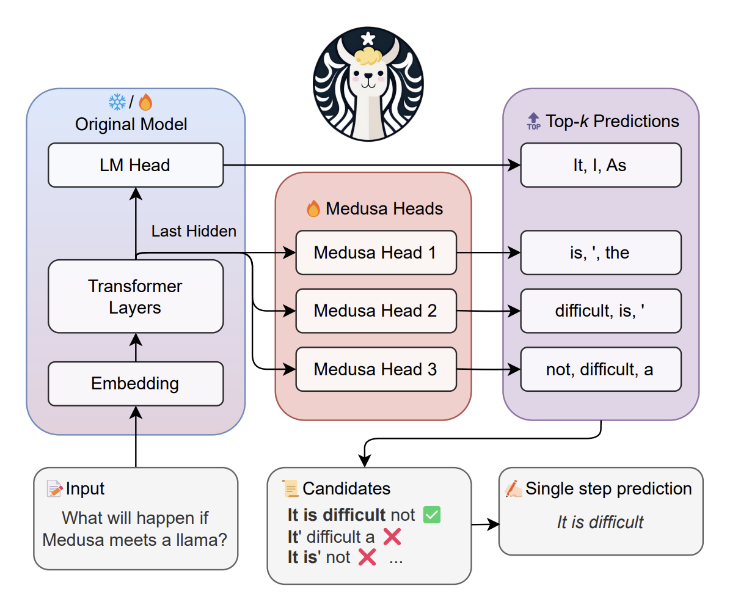
\includegraphics[width=0.75\textwidth]{Figures/fig2_medusa.png}
\caption[Medusa speculative decoding workflow]{Medusa speculative decoding workflow (reproduced from~\cite{cai2024medusa}).}
\label{fig:medusa}
\end{figure}

Another tree-based technique is EAGLE. Unlike Medusa, which predicts tokens independently, EAGLE shifts the drafting process to the feature level and performs it autoregressively. It observes that a more accurate prediction can be achieved by feeding the previous drafting step's feature back into the draft process~\cite{li2024eagle}. That drafting is carried out not by a separate small language model but by a single trained module, an FC layer followed by one decoder layer, which EAGLE calls its Autoregression Head. The EAGLE feature-based drafting process is depicted in Figure~\ref{fig:eagle}.

\begin{figure}[H]
\centering
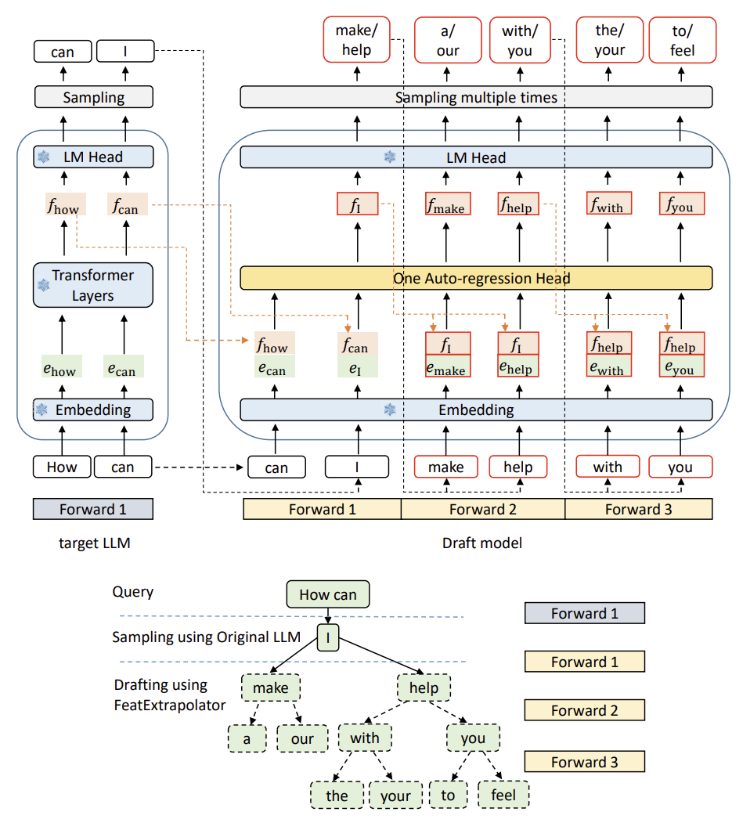
\includegraphics[width=0.75\textwidth]{Figures/fig3_eagle.png}
\caption[EAGLE speculative decoding workflow]{EAGLE speculative decoding workflow (reproduced from~\cite{li2024eagle}).}
\label{fig:eagle}
\end{figure}

EAGLE's draft tree has the same shape at every decoding iteration. EAGLE-2 starts from the observation that no single shape suits every context, since whether a draft token is accepted depends on the text being generated and not only on the token's position in the tree. A tree fixed in advance therefore spends nodes on branches the current context does not support. The second observation is that the EAGLE draft model is well-calibrated, meaning its confidence scores, the draft model's own output probabilities for each proposed token, closely approximate the true acceptance rates. For example, draft tokens with a confidence score below 0.05 are accepted only about 4\% of the time, whereas those above 0.95 are accepted roughly 98\% of the time~\cite{li2024eagle2}. EAGLE-2 does not vary the size of the draft tree; the total draft-token budget and tree depth are fixed. What is dynamic is which nodes fill that budget, and two separate steps decide it. The tree is grown one layer at a time, each expansion step feeding back only the highest-scoring nodes of the layer just added, where a node's score is the product of the draft probabilities along the path from the root to it. Once the tree reaches its full depth, every node in it is ranked by that same score, and the highest-ranked are the ones sent for verification. That fixed number of verified tokens is the speculative decoding length of Section~\ref{subsec:papi}. EAGLE-2 therefore spends the same token-level parallelism at every iteration, but on whichever branches the current context favours rather than on positions fixed in advance. An illustration of such a confidence-aware tree is shown in Figure~\ref{fig:eagle2}.

\begin{figure}[H]
\centering
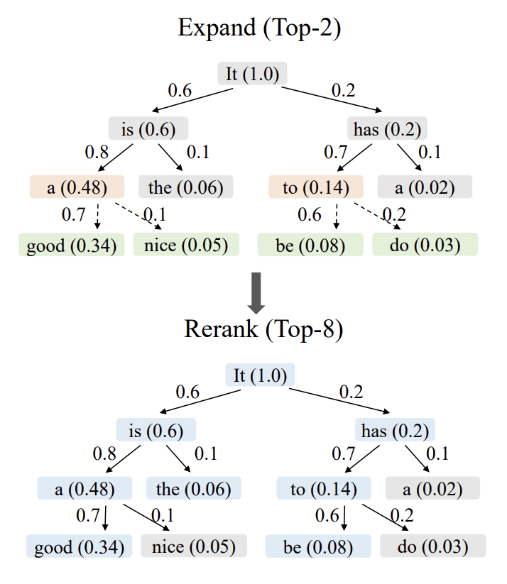
\includegraphics[width=0.55\textwidth]{Figures/fig4_eagle2_tree.png}
\caption[EAGLE-2 confidence-aware tree example]{EAGLE-2 confidence-aware tree example (reproduced from~\cite{li2024eagle2}).}
\label{fig:eagle2}
\end{figure}

This review does not catalogue every speculative decoding technique proposed since speculative sampling was first introduced~\cite{leviathan2023speculative}; the field is large and continues to grow. A comprehensive survey comparing a wide range of these techniques finds EAGLE the strongest performer it evaluates, ahead of Medusa and the other methods considered~\cite{xia2024survey}, and its successor EAGLE-2 improves on it further still~\cite{li2024eagle2}. The methods traced above therefore represent, to the best of our knowledge, the strongest tree-based drafting approach currently available, which is why this review focuses on them rather than surveying the field more broadly.

\subsection{LP-Spec: PIM-based LLM inference architecture for mobile devices}\label{subsec:lpspec}
LP-Spec is one of the state-of-the-art PIM-based architectures for on-device LLM inference. Unlike PAPI, which targets the server regime and exploits batching, LP-Spec addresses the mobile setting, where requests arrive one at a time and speculative decoding is the only remaining source of parallelism. It runs on a hybrid LPDDR5-PIM module built from three PIM ranks and one conventional DRAM rank, each four dies deep, for 16 GB of capacity in total. Near-bank compute inside the PIM ranks runs at 409.6 GOPS INT8 per die, an aggregate 4.9152 TOPS across all twelve PIM dies, reachable at 51.2 TB/s of internal bandwidth; the 51.2 GB/s external LPDDR5 bus remains available alongside it, letting the NPU read the same banks as ordinary DRAM instead. The mobile NPU it pairs with likewise splits its own compute across two units, a 32.8 TOPS matrix unit and an 8.2 TOPS vector unit~\cite{he2025lpspec}.

On top of Medusa speculative decoding, LP-Spec contributes two mechanisms: a Draft Token Pruner that trims the candidate tree before verification, and a Data Allocation Unit that divides verification between the PIM units and a mobile NPU to maximize speed. The overall architecture and its Draft Token Pruner are shown in Figure~\ref{fig:lpspec}~\cite{he2025lpspec}.

In Medusa speculative decoding, several additional decode heads each emit their top-k tokens, which are merged into a candidate token tree by sharing common prefixes. Verifying this entire tree in parallel is energy-intensive, so the Draft Token Pruner reduces it beforehand. For each decode head and candidate position, it maintains an acceptance-accuracy statistic estimated from previous verification results; a greedy expander then builds a smaller tree by repeatedly adding the node with the highest accuracy, while a hardware estimator keeps the tree within a performance and energy budget defined by its expected acceptance length. The number of candidates left standing once that budget is met, L\textsubscript{spec}, is what the tree offers verification each iteration. These accuracy statistics are refreshed after every decoding iteration from the latest verification outcomes, so the pruned tree is optimized at run-time from accumulated historical statistics~\cite{he2025lpspec}.

To execute verification, LP-Spec partitions the workload between the NPU and the PIM units using column-wise tensor parallelism, with the model weights and KV-cache distributed across the PIM and DRAM ranks. Both the FC and the attention layers are split across the two units in this manner. The PIM hardware verifies candidate tokens four at a time, across four 32-wide SIMD ALUs ($N_{\text{ALU}} = 4$) built into its compute units; a tree with more surviving candidates than that needs a further pass, so PIM throughput rises in steps with the tree's size rather than smoothly. The Data Allocation Unit accounts for this by recomputing the partition ratio for each decoding iteration from the current speculation length, L\textsubscript{spec}, continuously adjusting how much of the verification is mapped to the NPU versus the PIM rather than committing each layer to a single device~\cite{he2025lpspec}.

\begin{figure}[H]
\centering
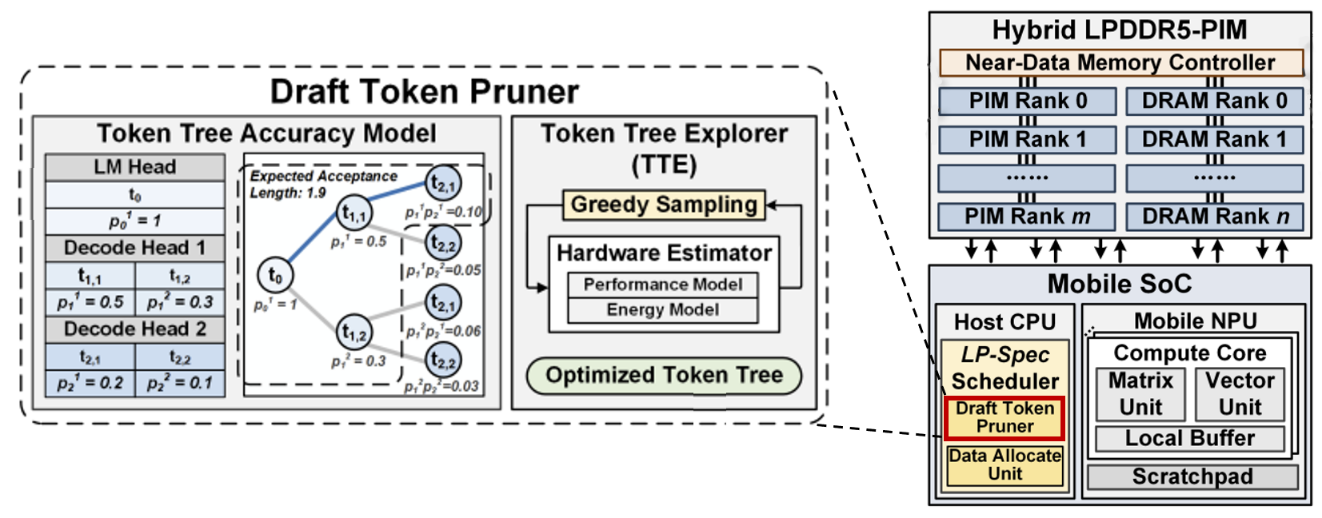
\includegraphics[width=\textwidth]{Figures/fig6_lpspec.png}
\caption[LP-Spec architecture and Draft Token Pruner]{LP-Spec architecture and Draft Token Pruner (reproduced from~\cite{he2025lpspec}).}
\label{fig:lpspec}
\end{figure}


% ---------- Chapter Three ----------
\newpage
\section{Problem Statement}

\subsection{Motivation}
LLMs have achieved tremendous success across a variety of domains, and there is growing demand to run them directly on mobile and edge devices rather than in the cloud. On-device execution keeps user data local, avoids the network delay and jitter incurred by cloud round-trips, and preserves service availability without depending on a connection. However, deploying LLMs at the edge remains fundamentally constrained: a model must stream its full set of weights from memory for every token it generates, and edge platforms offer only a fraction of the memory bandwidth and energy budget available in the data centre~\cite{chen2026edge}.

These constraints make efficient on-device inference an acute and increasingly studied problem. The first of them is energy. A mobile device draws from a fixed battery that must simultaneously serve the display, connectivity, and the everyday applications for which the device is primarily used. Inference therefore competes for an energy budget it does not own. That budget is exhausted quickly: under continuous inference with a 4-bit quantized 3B model, a smartphone's battery is estimated to be depleted after roughly 490--590 prompts~\cite{laskaridis2024melting}. Crucially, that energy is not spent where one might expect. In a processor-centric system, the weights are stored in memory and must be brought to the compute units before they can be used, and it is this movement, rather than the arithmetic performed once the data arrives, that dominates. When large commercial neural-network models are executed on modern edge machine learning accelerators, more than 90\% of the entire system energy is consumed by memory rather than by computation~\cite{mutlu2022primer}. For this class of workload, energy efficiency, rather than peak compute, is therefore the primary objective, and reducing data movement is the most direct means of improving it. This is precisely what PIM offers: by placing compute units next to the DRAM banks, weights are processed where they reside instead of being moved across an external bus.

The second constraint is speed. An LLM generates its output sequentially, one token at a time, and in a processor-centric system each of these tokens requires the model's full set of weights to be moved across the off-chip interface. Commodity edge hardware provides only tens of GB/s for this transfer, far below that of server accelerators~\cite{chen2025elib}. In the data centre, this cost is amortized by batching: a single fetch of the weights serves many sequences at once. On-device inference, however, serves a single user stream and is therefore restricted to a batch size of one. This leaves speculative decoding as the primary source of parallelism, which attacks decoding latency by drafting several candidate tokens and verifying them in parallel.

Research on efficient mobile LLM inference should therefore prioritize PIM-based architectures that specifically exploit speculative decoding, since the two techniques address the two constraints in a complementary manner.

\subsection{Problem definition}
LP-Spec, one of the current state-of-the-art mobile PIM architectures for LLM inference, adopts Medusa speculative decoding. To bound the energy cost of speculation, it prunes the draft tree as the tree is built, keeping the branches most likely to be accepted. A hardware estimator caps how many branches survive, sizing the tree to an energy and performance budget, so a scarcer budget yields a smaller tree. It selects the branches to keep from per-(head, position) acceptance accuracies accumulated over previous decoding iterations -- a property of the draft heads and their history~\cite{he2025lpspec}. More recent speculative decoding methods outperform Medusa: in an independent evaluation of drafting techniques, EAGLE achieves the highest speedup across the settings considered~\cite{xia2024survey}, and its successor EAGLE-2 is faster still~\cite{li2024eagle2}, shaping its draft tree from per-token confidence scores computed for the current context. It uses these scores to decide which branches to expand, but not when to stop expanding. The draft tree therefore grows to a fixed size, the same whether or not the model is confident in the context. No mobile PIM architecture has yet adopted this family of methods. Because EAGLE-2's scores are tied to the context being generated, they might serve as a more accurate pruning criterion than LP-Spec's retrospective one, pruning fewer tokens that would have been accepted and more that would have been rejected.

Pruning is not the only run-time decision such an architecture makes. It must also route the verification workload between the PIM and the NPU; drafting, a single parallel pass under Medusa, is light enough to set aside here. LP-Spec's Data Allocation Unit partitions each layer column-wise between the NPU and the PIM, so the two devices verify concurrently. It reads the ratio of that split from an allocation table indexed by the draft tree's size, choosing the value that synchronizes the two units' execution times~\cite{he2025lpspec}. The Data Allocation Unit's objective is therefore latency; energy was weighed when the tree was sized, but not when the work is placed. Since the NPU always carries work, a share of the weights crosses the off-chip interface on every pass. That crossing is where most of the pass's energy goes, because moving a weight off-chip costs several times more energy than accessing it in memory. On a low battery, the slower in-memory placement the Data Allocation Unit never selects may be the better one to run -- a trade-off a latency objective cannot make.

EAGLE-2's confidence scores could inform both of these decisions, though only the first directly. As a pruning criterion, the scores supply the stopping rule the fixed-size tree lacks: a branch stops expanding when its score falls below a threshold, so the tree stops growing where the model's confidence runs out. Its size then follows the context -- a confident context supports a large tree, an uncertain one a small tree. LP-Spec prunes to the same end, sparing the energy of verifying tokens unlikely to be accepted; a confidence gate might achieve that more naturally, since the scores that size the tree are computed during the drafting itself. The dynamic tree size could in turn decide placement. A small tree carries little verification work and may be better kept in memory, while a large one may justify the off-chip crossing for the NPU's speed.

This leads us to the following research questions:
\begin{enumerate}
    \item Can a PIM-based LLM inference architecture for mobile devices natively adopt EAGLE-family speculative decoding, and outperform the existing state-of-the-art architecture?
    \item Can EAGLE-2's per-token confidence scores serve as a live, context-aware criterion for pruning the draft tree?
    \item Can the size of the resulting draft tree route verification between the PIM and the NPU, trading energy against latency according to the device's battery and thermal state?
\end{enumerate}

\subsection{Objectives}
\label{subsec:objectives}
The primary objective of this project is to propose and simulate a novel confidence-aware PIM-based architecture for LLM inference on mobile devices. This will be achieved through the following specific objectives:
\begin{itemize}
    \item \textbf{Characterize EAGLE-2's draft-tree behavior:} Study how EAGLE-2 constructs and scores its draft trees during decoding. Identify a confidence-based pruning criterion and threshold that a mobile LLM inference system can act on, saving energy by reducing verification of tokens unlikely to be accepted.
    \item \textbf{Develop a dynamic routing policy:} Formulate a PIM-NPU scheduling policy that routes verification of the pruned candidate tree between PIM and NPU according to its size.
    \item \textbf{Design the CAPIM control architecture:} Develop the control logic that runs EAGLE-2 inference under confidence-based pruning and the routing policy above. Make both configurable at runtime, so the threshold can shift to a low-power mode under battery or thermal constraints.
    \item \textbf{Evaluate via simulation:} Build a simulation environment for CAPIM and the baseline architectures, sharing a common cost model so comparisons are fair, and use it to quantify latency and energy-efficiency improvements over the state of the art. The improvement sought over LP-Spec is 20--30\% in energy efficiency and 1.5×--2× in throughput.
\end{itemize}


% ---------- Chapter Four ----------
\newpage
\section{Methodology}

\subsection{Architecture overview}
\label{sec:overview}
Chapter 3 set out three research questions. The first asks whether a mobile PIM architecture can natively adopt EAGLE-family in place of LP-Spec's Medusa speculative decoding. The second asks whether EAGLE-2's per-token confidence scores can serve as a live, context-aware criterion for pruning the draft tree. The third asks whether the size of the resulting tree can route verification between PIM and the NPU. This section sets out the architecture proposed to address them: how its dedicated controller is placed alongside the existing PIM and NPU substrate, the dataflow it executes at every decoding iteration, and the two run-time thresholds that control that dataflow. The pruning criterion, the routing policy, and the controller that carries both out are each developed in full in Sections~\ref{sec:gate}, \ref{sec:routing} and \ref{sec:controller}; what follows here is the architecture-level account those sections build on.

CAPIM keeps LP-Spec's PIM and NPU substrate as given, since neither device is this project's contribution, and instead replaces the control logic built on top of them. The Draft Token Pruner and the Data Allocation Unit's per-iteration partition choice are both replaced by a single dedicated controller, placed alongside the host CPU and the NPU with the same direct access to the hybrid LPDDR5-PIM. Figure~\ref{fig:capim-soc} shows this placement, together with the controller's internal structure, which Section~\ref{sec:controller} develops in full; what follows here is the dataflow that controller executes.

\begin{figure}[H]
\centering
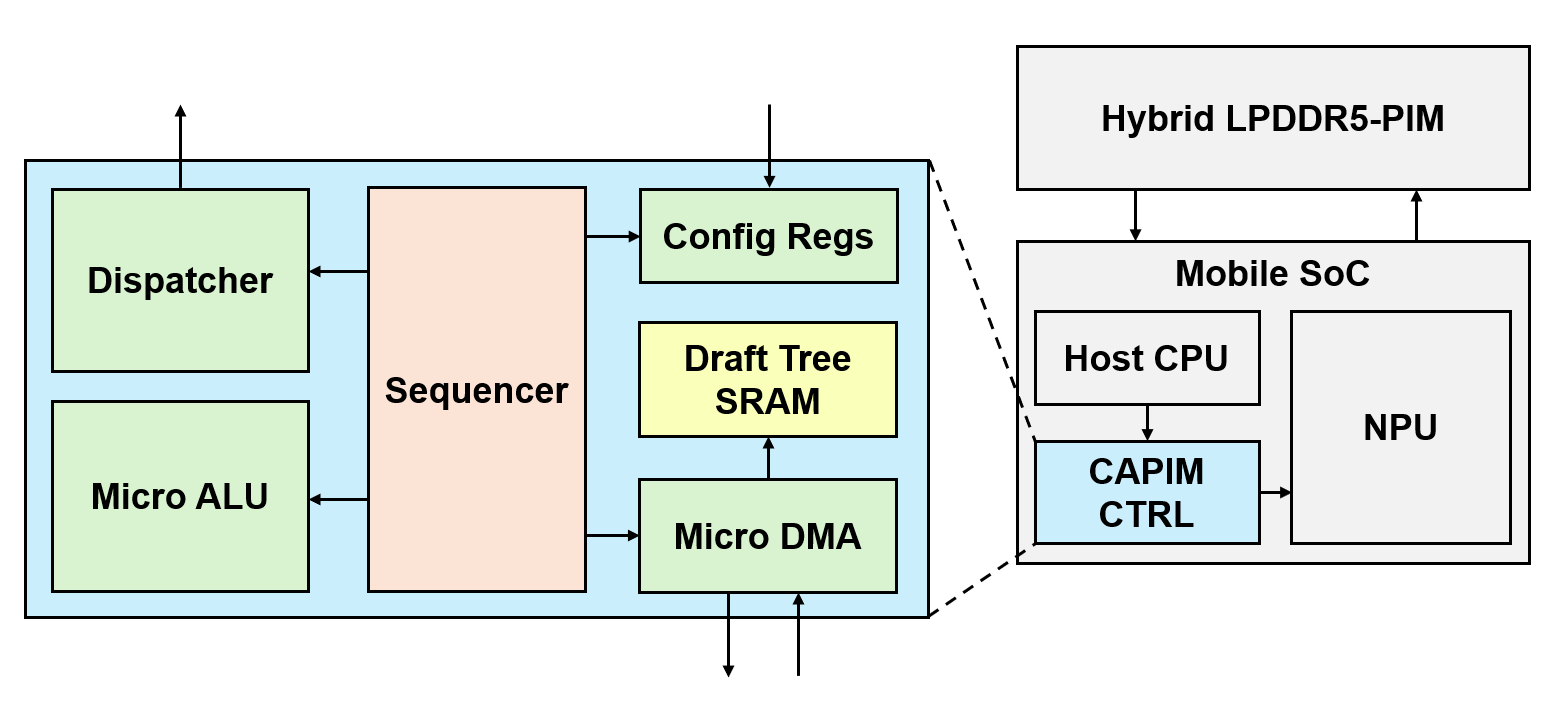
\includegraphics[width=\textwidth]{Figures/CAPIM-architecture.PNG}
	\caption{CAPIM's architecture and the controller internal structure}
\label{fig:capim-soc}
\end{figure}

Figure~\ref{fig:capim-dataflow} shows the dataflow once for prefill and once for the decode loop that follows it, with every stage tagged to the device that executes it. Prefill runs once, on the NPU, as a single high-parallelism, compute-bound pass over the prompt; it writes the resulting KV-cache into the PIM banks and produces the target model's hidden features for the prompt's last position, which seed the first decoding iteration's drafting. Every decoding iteration thereafter repeats the same stages, and each one reseeds the next. The target model's verification pass produces fresh hidden features for whichever tokens it accepts, and those seed the following iteration's draft. Drafting itself runs mostly on PIM. EAGLE-2's draft model is a lightweight autoregressive decoder in its own right, and it grows the candidate tree one expansion step at a time. Its linear kernels -- the QKV and feedforward projections, and the attention score and context matrix multiplications run on PIM; only its non-linear operations -- RMSNorm and softmax -- are handed to the NPU at each step. After each expansion step, a controller (\textsc{capim ctrl} in the figure, developed fully in Section~\ref{sec:controller}) checks the confidence accumulated along every surviving branch against a threshold, σ\textsubscript{th}, and any branch that falls below it is stopped immediately rather than expanded again. This repeats until drafting is judged complete, at which point the same controller compares the size of the surviving tree, μ, against a second threshold, μ\textsubscript{th}. That comparison decides where verification runs: a tree smaller than μ\textsubscript{th} has its verification pass offloaded to PIM as far as the near-bank datapath allows, while a tree at or above it has its FC kernels column-split between PIM and the NPU instead; attention's matrix multiplications stay on PIM regardless of which route is taken. Non-linear operations are handed to the NPU in both routes. The tokens verification accepts become the seed for the next decoding iteration's drafting, and the loop repeats.
 

\begin{figure}[H]
\centering
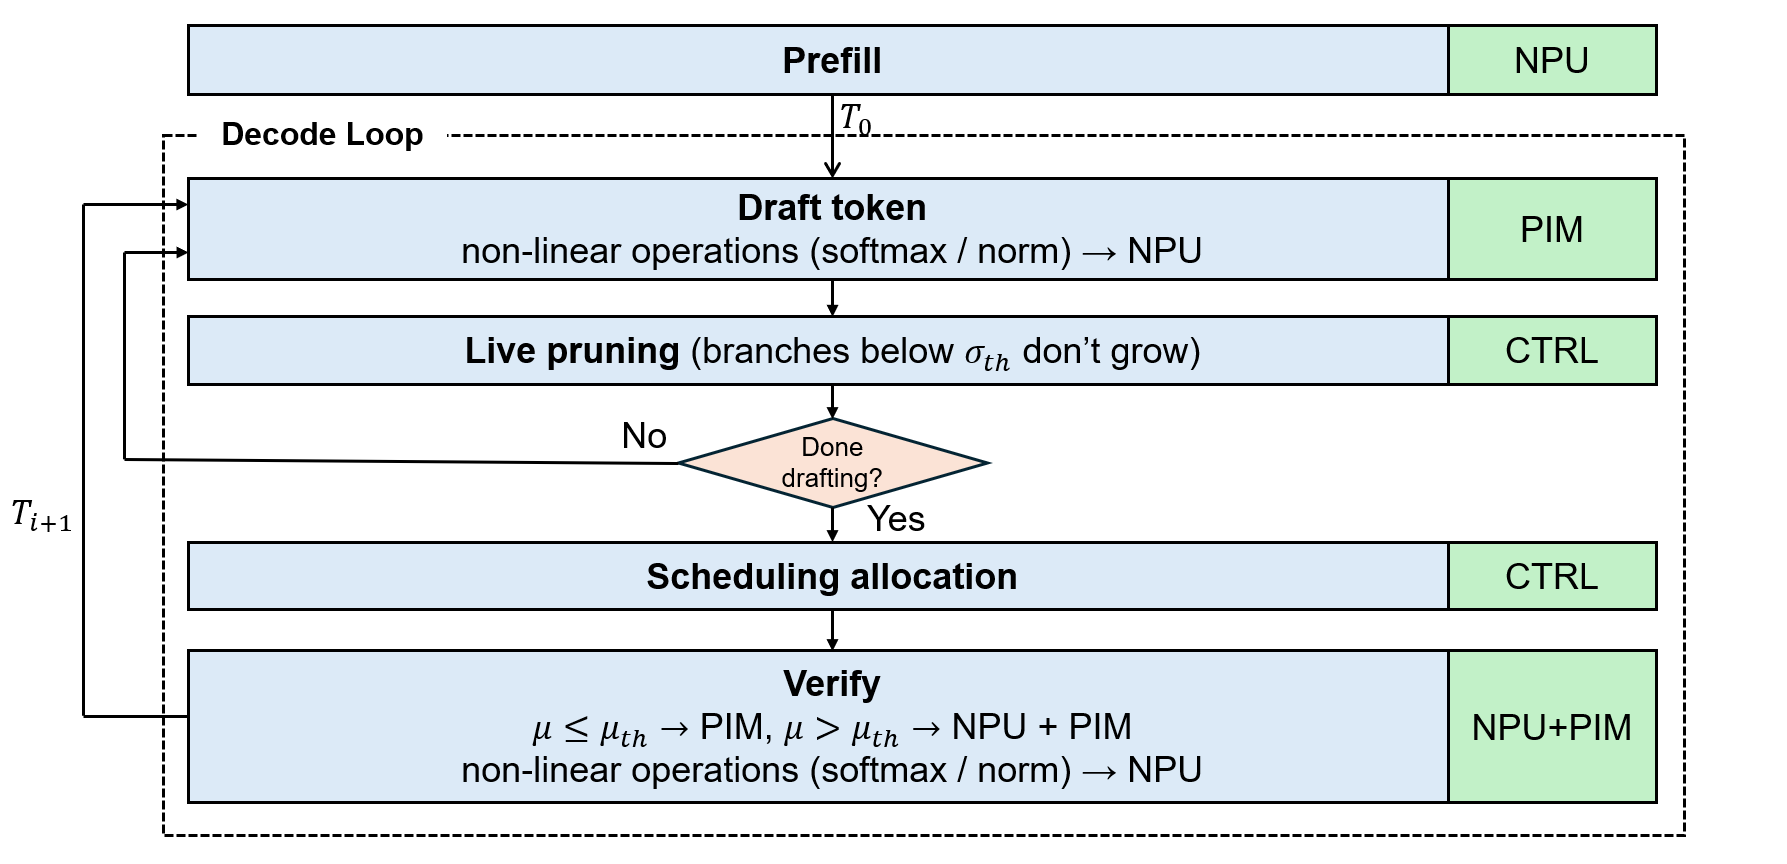
\includegraphics[width=\textwidth]{Figures/CAPIM-inference-flow.png}
\caption{CAPIM's device-tagged inference flow}
\label{fig:capim-dataflow}
\end{figure}

Two thresholds are introduced by name in the walkthrough above and used throughout the rest of this chapter. σ\textsubscript{th} is a threshold on cumulative log-probability: the sum of the log-probabilities assigned to every token on the path from the tree's root to a given node, compared against a fixed value each time a branch is about to be expanded again. μ\textsubscript{th} is a threshold on tree size: the number of surviving nodes μ, compared once, after drafting ends, against a fixed count. Both are architected as run-time controls rather than values fixed at design time. The CAPIM Controller holds each as a configuration register the host can rewrite before a request, described in Section~\ref{sec:controller}.

Both mechanisms replace a corresponding piece of LP-Spec, described in Section~\ref{subsec:lpspec}. σ\textsubscript{th} replaces LP-Spec's Draft Token Pruner with a judgement drawn from the current context, stopping or keeping each branch on the confidence the draft model assigns to it as it is drafted, so a confident context and an uncertain one are not pruned to the same tree size. μ\textsubscript{th} replaces the unconditional split LP-Spec's Data Allocation Unit always performs with a threshold, turning whether a tree is split at all into a decision rather than a certainty.

\subsection{Model's confidence-based pruning}
\label{sec:gate}
The confidence gate is a per-node check performed as EAGLE-2's draft model produces each node. A node is drafted at all only if its parent was itself drafted and survived the check; once drafted, its own cumulative score is compared against σ\textsubscript{th}. A node whose score survives the check is expanded normally, and its children become candidates at the next depth. A node whose score does not is a boundary: it is still drafted, since a node's score can only be known once it exists, but nothing is drafted from it in turn -- its children are never generated. What the gate saves is therefore not the boundary node's own cost, which the check cannot avoid, but every node beyond it that a fixed-size tree would otherwise have drafted, scored, and sent to verification.

CAPIM does not need a new signal for the gate, because building an EAGLE-2 tree already produces one. That signal is the cumulative confidence score, accumulated along the path from the root of the tree to a node. Section~\ref{subsec:sd} described the two selections EAGLE-2 makes with it: which nodes of the newest layer to expand, and which of the finished tree to verify. σ\textsubscript{th} is compared against that same score, and it replaces both. What EAGLE-2 does with the number is not what CAPIM does with it. Each of its selections takes a fixed count of the highest-scoring candidates, so each is a relative judgement, comparing candidates only against each other to fill a budget set in advance. σ\textsubscript{th} instead judges a branch on its own, with nothing else to compare it against, stopping it once its score falls too low to continue -- an absolute judgement. The tree that survives the gate is the tree sent for verification, so there is no second selection to make, no fixed budget for it to fill, and no ranking of every drafted candidate to carry out. Whether the accumulated score is calibrated well enough to support that judgement is tested empirically, by the method in Section~\ref{sec:characterization} and the result in Section~\ref{sec:pruning}.

Making that judgement is nonetheless cheap to build, for three reasons intrinsic to the score itself. First, extending a path by one more token can only ever add that token's own log-probability, which is never positive; a node's cumulative score can therefore only fall or hold as the path grows, never rise, making it monotonically non-increasing with depth. Second, this makes the surviving set ancestor-closed without any extra bookkeeping, because a node's score is always at most its parent's. Consequently, a node cannot clear σ\textsubscript{th} unless its parent did too, ensuring that the nodes kept at any depth are automatically connected back to the root. Third, the check itself needs no memory of the path. Since ancestor-closure is guaranteed by construction, a node's survival depends only on its own score and whether its immediate parent survived, not on re-examining every ancestor in turn. A single running comparator per branch is therefore enough; no pass or fail result need propagate through the tree.

\subsection{Tree size-based routing}
\label{sec:routing}
μ\textsubscript{th} decides where the verification pass over the drafted tree is run. It is a single decision, made once per iteration after drafting ends, unlike σ\textsubscript{th}'s per-node check. Having tracked how many nodes survive as the tree is grown and pruned, the controller compares that count, μ, against the threshold, and the outcome selects between the two verification routes below.

A tree smaller than μ\textsubscript{th} takes the sequential route. Every kernel in the verification pass -- the FC kernels and the attention kernel alike -- is offloaded to PIM, and the non-linear operations between them are handed to the NPU. No two kernels run at once, so the pass's latency is the sum of every kernel's own cost. Section~\ref{subsec:papi} showed an FC kernel's arithmetic intensity grows with the product of the batch size and the speculative decoding length. CAPIM's batch-size-one mobile setting fixes the first term at one, so that product reduces to the second term alone -- and μ, the surviving tree size, is that term at CAPIM's operating point. A tree below μ\textsubscript{th} therefore keeps μ small enough to leave the FC kernels in the memory-bound regime PIM's near-bank bandwidth is built for.

A tree at or above μ\textsubscript{th} takes the concurrent route instead, but only for the FC kernels. They are column-split between PIM and the NPU. Each device computes a disjoint share of the output columns over the same broadcast input, and the split is balanced so that both shares finish together -- the same balanced-makespan construction LP-Spec's own Data Allocation Unit uses for its own split (Section~\ref{subsec:lpspec}). CAPIM does not extend that split to the attention kernel. Section~\ref{subsec:papi} established that the attention kernel is always memory-bound, regardless of the parallelism available to it. This is unlike the FC kernels, whose regime shifts with the same speculative decoding length μ now instantiates. There is therefore no μ at which splitting attention between PIM and the NPU would be worthwhile, so its matrix multiplications stay on PIM in both routes. Non-linear operations are handed to the NPU in this route exactly as in the sequential one; only the FC kernels' device, and whether they run sequentially or concurrently, change with the threshold.

\subsection{The CAPIM controller}
\label{sec:controller}
The CAPIM Controller is a self-contained engine that runs the decoding loop from end to end. The host writes its configuration and a start bit once per request, then takes no further part until the controller interrupts it, which is what lifts the loop's per-kernel control off the host. The controller supplies that control and nothing else. It issues commands to PIM and to the NPU and evaluates the two scalar predicates behind σ\textsubscript{th} and μ\textsubscript{th}, while every FC, attention and non-linear kernel still executes on one of those two devices. Its six blocks are shown on the left of Figure~\ref{fig:capim-soc}. The sequencer is the only one that decides anything; the other five carry out what it issues.

\begin{itemize}
    \item \textbf{Sequencer:} the finite-state machine that drives the loop. It sequences prefill, drafting, verification and acceptance, and takes the decisions those stages turn on -- whether a branch survives the gate, which route verification takes, and whether drafting continues.
    \item \textbf{Draft tree SRAM:} the sequencer's working state, the draft tree itself. For every live node it holds a parent pointer, token id, cumulative log-probability, an alive flag and a depth. EAGLE-2 fixes its draft-token budget in advance (Section~\ref{subsec:sd}), so the store is sized to that budget and the gate only ever keeps the live tree below it. It sits on-chip because the sequencer re-reads it at every expansion step.
    \item \textbf{Config registers:} a passive file the host writes once per request -- pointers to the weights, the KV-cache and the output buffer, and both thresholds σ\textsubscript{th} and μ\textsubscript{th} -- before raising the start bit that wakes the sequencer. The sequencer reads it throughout.
    \item \textbf{Dispatcher:} turns a sequencer directive into the command each device expects -- a stream of commands against a preloaded microprogram for PIM, a descriptor and a doorbell write for the NPU -- and issues it without waiting on the result.
    \item \textbf{Micro DMA:} moves data between the controller and memory. It writes the results a device returns, confidence scores and accept bits, into the nodes already held in the draft tree SRAM, and commits accepted token ids out to the output buffer.
    \item \textbf{Micro ALU:} a single shared adder-comparator, time-multiplexed across accumulating a node's cumulative log-probability, comparing it against σ\textsubscript{th}, and comparing the surviving tree's size against μ\textsubscript{th}.
\end{itemize}

The controller's operation over a single request follows the dataflow Section~\ref{sec:overview} set out, now attributed to the blocks that carry it out. Once the host writes its configuration and the start bit, the sequencer wakes, dispatches prefill to the NPU, and writes the resulting root node into the draft tree SRAM. Drafting then proceeds one expansion step at a time. The sequencer directs the dispatcher to issue that step's FC and attention kernels to PIM, and the resulting logits go to the NPU for the softmax the confidence score requires. What returns is only a small number of scalars, each surviving candidate's token id and log-probability, resolved by the NPU's own top-k selection over the distribution its softmax produces. The micro ALU accumulates each candidate's cumulative log-probability and compares it against σ\textsubscript{th}; the sequencer applies the result to the tree, keeping the survivors and marking the rest dead, and tests whether to expand again. Every one of these exchanges is an issue followed by a wait, the dispatcher returning as soon as the command is out and the sequencer idling until the device's done-signal releases it.

Drafting ends when no branch survives the gate to expand, or when the tree reaches the depth EAGLE-2 fixes. The sequencer reads the surviving tree's size and the micro ALU compares it against μ\textsubscript{th}, selecting one of the two verification routes Section~\ref{sec:routing} set out. Carrying that choice out is purely a dispatch difference. Below μ\textsubscript{th}, the dispatcher issues one command per kernel -- the FC and attention kernels to PIM, the non-linear operations between them to the NPU -- and the sequencer waits on a single done-signal each time. At or above it, the FC kernels are instead issued as one paired PIM-and-NPU command carrying the column split LP-Spec's Data Allocation Unit performs, and the sequencer stays idle until both done-signals arrive. Attention and the non-linear operations are issued the same way either side of the threshold.

The accept test runs as the final step of the NPU's verification pass and returns a per-node accept bit, which the micro DMA pulls back into the draft tree SRAM. From those bits the sequencer walks the tree once, from the root, to find the longest accepted prefix and the nodes that seed the next draft. The micro DMA appends the accepted token ids to the output buffer, and the sequencer raises an interrupt marking those tokens ready before resetting the tree to those nodes and returning to drafting. The cycle repeats until the request ends, at which point the sequencer raises a completion interrupt instead and the host wakes to read the result.

\subsection{Evaluation overview}
\label{sec:approach}
Sections~\ref{sec:overview}--\ref{sec:controller} specified the architecture in full, from its dataflow to the two thresholds that control it and the controller that carries both out. What remains is a method that can say whether that architecture is worthwhile, without fabricating hardware to find out. It must predict the latency and energy a design would show. It must also measure every design it compares in the same way, so that any difference between them reflects the designs and not how they were assessed. CAPIM and the LP-Spec baseline are held to that measurement, together with a plain autoregressive decoder as a lower bound. The approach adopted is trace-driven analytical simulation, carried out in three stages: EAGLE-2's drafting behaviour is characterized and a pruning criterion drawn from it; that criterion, and the baseline's own pruner, are then swept over a range of settings during real decoding, producing a family of traces that record how each architecture behaves once pruned at each setting; and each of those traces is finally priced on a shared analytical cost model, sweeping the remaining open routing threshold.

Recording the model's behaviour once and simulating over the recording, rather than running the model inside every experiment, is what keeps the sweeps of the last two stages affordable. Model inference requires a GPU and dominates the cost of a run, whereas the analytical simulation is inexpensive and runs on a CPU. The design space has two thresholds to sweep, one on confidence and one on routing, alongside the placement choices weighed as the architecture was designed. Re-running the model at every point in it would have needed more GPU time than was available. Recording a bounded family of decoding behaviours once instead lets every point be evaluated on a CPU, so the costly measurement is paid for a fixed number of times and the exploration that follows is cheap.

The LP-Spec baseline could not be obtained from its authors. Its simulation framework is not published, and a request for it went unanswered, so no part of its implementation was available to build on. Everything the baseline needs is therefore reconstructed from the paper's description. Its Draft Token Pruner is rebuilt, so that Medusa's decoding can be recorded with that pruner shaping its trees. Its execution model is rebuilt as a driver, so that those recordings can be priced.

The first of the three stages searches for the criterion the gate needs, by examining how EAGLE-2 scores the tree it drafts and whether those scores match which of its nodes the target model accepts when it verifies them. It is specific to CAPIM, and has no counterpart in the baseline. The method behind this stage, and the instrumentation it and the next stage both rely on, are given in full in Section~\ref{sec:characterization}.

The second stage records how each architecture decodes once its own pruning is genuinely in effect, and here CAPIM and the baseline are treated alike. Both reuse the instrumentation Section~\ref{sec:characterization} introduces, now run with the pruning active rather than merely observing. CAPIM's confidence threshold is applied inside EAGLE-2's decoding loop as the tree is drafted, and LP-Spec's retrospective pruner is applied the same way inside Medusa's. A branch either mechanism discards is therefore removed before the target model ever sees it. Sweeping a mechanism's threshold this way -- σ\textsubscript{th} for CAPIM, L\textsubscript{spec} for LP-Spec -- yields a family of traces, one per setting. Because the pruning happens inside the decoding call itself, rather than being applied to a recording afterwards, each trace is the trajectory that mechanism genuinely produces at that setting. A token the gate discards changes the context every later step decodes from, exactly as it would on real hardware.

The third stage turns those traces into latency and energy figures. A single analytical cost model prices the individual layers of a transformer, and each architecture -- autoregressive decoding, LP-Spec, and CAPIM -- is expressed as a thin driver that emits its layers and composes them according to its own execution model. Because all three are priced by the same model, any difference in their results comes from the designs themselves and not from how each was costed. One quantity is still open when a trace reaches this stage. μ\textsubscript{th}, the routing threshold, decides where each verification pass runs without altering what the trace recorded, so it is swept as each trace is priced -- σ\textsubscript{th} and L\textsubscript{spec} having already been swept during collection. Both thresholds are configuration registers the controller reads at run time, so the evaluation reports the range each can take rather than fixing one setting as the design. The model itself, and the hardware it represents, are given in Section~\ref{sec:costmodel}.

The implementation of all three stages -- the instrumented collectors, the shared cost model and its three drivers, and the scripts that generate every table and figure in this report -- is available at \url{https://github.com/idanhochman/capim}.

\subsection{Collecting and pruning draft trees}
\label{sec:characterization}
This section sets out how the draft trees were logged, and how each method's pruning was applied inside the decoding loop that produced them. Two methods are instrumented, EAGLE-2 for CAPIM and Medusa for the LP-Spec baseline, and the instrumentation takes the same form in each. Functions inside the decoding loop are wrapped so their inputs and outputs can be read as the model runs. What those wrappers see is logged as one entry per drafted node, giving that node's position in the tree, its cumulative confidence score where the method computes one, and whether the target model accepted or rejected it at verification. The same wrappers produce both kinds of trace the evaluation needs, run either with a pruning threshold active or without one. Those traces are what the analysis of EAGLE-2's drafting behaviour rests on, and what drives the cost model for CAPIM and for both baselines. What is wrapped in each, and how it behaves in either mode, is set out below.

The EAGLE-2 traces are collected by running its authors' own implementation and reading what its decoding loop already computes. Two functions in that loop are wrapped, and neither function's own logic is changed. One builds a decoding iteration's entire draft tree, working through every expansion step internally before returning the candidate token ids, the tree structure connecting them to their parents, and the path table the decoding loop walks during verification. The cumulative scores are not returned alongside them, being internal to how that function ranks its candidates. It is therefore rebound at load time to a copy of itself carrying one extra line that saves the scores as they are computed, so that the gate can read them back without the authors' own code being altered. The other wrapped function applies EAGLE-2's own acceptance rule to that path table, deciding how many of a verified tree's tokens the target model accepts. Wrapping it is what makes each node's outcome observable: reading what it returns is how every drafted node in a trace comes to be labelled accepted or rejected. With no threshold applied, the path table passes through untouched, and a node's confidence score, tree position and eventual accept/reject outcome are all recorded together once the acceptance function runs. With a threshold active, the first wrapper additionally edits the path table before returning it. Any path through a node whose score falls below σ\textsubscript{th} is truncated at that node, exactly as the confidence gate does. The acceptance function then runs unmodified on the edited table, so it can only ever accept along a surviving path -- a pruned branch is cut before verification ever sees it, without the acceptance rule itself changing.

The traces the LP-Spec baseline runs on are collected the same way, from Medusa's own implementation, and they record the same per-node data with one omission. A Medusa node carries no confidence score, so only its position in the tree and its eventual accept/reject outcome are logged. Two of Medusa's functions are wrapped to obtain them. The first builds a decoding iteration's candidate tree, populating Medusa's fixed structure with the iteration's tokens and the path table the verifier walks. The second applies Medusa's acceptance rule to that path table, and reading what it returns is what labels each candidate accepted or rejected. Pruning is inserted into the first wrapper, between building the tree and handing it on. LP-Spec's Draft Token Pruner selects which candidates to keep, and the path table is edited to remove the rest before the verifier ever sees them. The pruner works retrospectively: it scores each position in the tree by the acceptance rate it has shown over previous iterations, and keeps the highest-scoring. After each iteration its outcomes are folded back in, so the statistics guiding one iteration reflect every iteration before it. The pruner is the reconstruction described above, run inside the decoding loop. The number of candidates it keeps, L\textsubscript{spec}, is the knob swept to produce the family of baseline traces, and at its largest setting it retains the whole static tree and prunes nothing, giving the baseline's unpruned trace.

\subsection{Cost model}
\label{sec:costmodel}
A single cost model produces every latency and energy figure the evaluation reports, for CAPIM and for both baselines alike, so that whatever differs between them is the design and not the instrument measuring it. It is organised as one shared layer model and three thin drivers. The layer model decomposes a transformer's decoding step into a small set of typed layers -- weight-stationary GEMMs (QKV, projection, the feedforward network, the LM head), the weightless attention matrix multiplications, and the non-linear glue between them (softmax, RMSNorm) -- and prices each layer once it is told which device runs it. Autoregressive decoding, LP-Spec, and CAPIM are each a driver that emits this same layer list, tagged with a device per layer, and composes the tagged layers into a step latency according to its own execution model -- sequential for autoregressive decoding, a concurrent makespan for LP-Spec, and the μ\textsubscript{th}-conditioned mix of the two that Section~\ref{sec:routing} already described for CAPIM. Sharing one layer model is what carries that fairness through to the hardware evaluation.

A typed layer's latency follows a per-layer roofline, the same form on either device:
\begin{equation}
t_{\text{layer}} = \max\!\left( \frac{c_{\text{layer}}}{\Pi_{\text{device}}},\ \frac{b_{\text{layer}}}{B_{\text{device}}} \right)
\label{eq:roofline}
\end{equation}
where $c_{\text{layer}}$ is the layer's operation count and $\Pi_{\text{device}}$ the device's peak compute throughput, $b_{\text{layer}}$ the bytes it must move and $B_{\text{device}}$ the relevant bandwidth -- PIM's internal bank bandwidth for a kernel it runs and the shared external bus for the NPU. A layer is compute-bound or memory-bound according to which term of Equation~\ref{eq:roofline} wins. PIM's compute term carries one further subtlety. Its near-bank ALUs are token-parallel, so a single pass over the weights verifies up to $N_{\text{ALU}}$ nodes at once, and the term therefore rounds a tree of μ nodes up to the next multiple of $N_{\text{ALU}}$ and counts whole passes. This organisation is part of the PIM substrate LP-Spec proposed, adopted here unchanged, since CAPIM's contribution is the confidence-driven control above it rather than the memory microarchitecture beneath.

A layer's energy comes from two sources, the bits it moves and the operations it performs. The first is charged at a fixed cost per bit for the interface crossed, the second at a fixed cost per operation. Both figures are taken from published sources rather than produced by a simulator. This mirrors LP-Spec, which models performance analytically and draws its energy from prior work~\cite{he2025lpspec}. It is in any case the only option available. No public simulator accurately models commercial LPDDR5-PIM, the existing ones being limited to generic HBM or DDR memory~\cite{cha2026lp5x}.

Table~\ref{tab:costparams} lists every constant that Equation~\ref{eq:roofline} and the energy model draw on. The throughput and bandwidth figures come from LP-Spec's own reported platform, so both designs are priced against the same device parameters. What differs between them is therefore the control logic, not the substrate it runs on. The movement and compute energy figures come from AttAcc, LP-Spec's own cited source for these figures~\cite{park2024attacc}.

\begin{table}[H]
\centering
\footnotesize
\begin{tabular}{lll}
\toprule
Parameter & Value & Source \\
\midrule
PIM INT8 compute per die & 409.6 GOPS & \cite{he2025lpspec} \\
PIM dies & 12 & \cite{he2025lpspec} \\
PIM internal bandwidth & 51.2 TB/s & \cite{he2025lpspec} \\
Shared external bandwidth & 51.2 GB/s & \cite{he2025lpspec} \\
PIM ALUs per pass ($N_{\text{ALU}}$) & 4 & \cite{he2025lpspec} \\
NPU INT8 matrix throughput & 32.8 TOPS & \cite{he2025lpspec} \\
NPU vector throughput & 8.2 TOPS & \cite{he2025lpspec} \\
In-bank movement energy & 0.55 pJ/bit & \cite{park2024attacc} \\
Off-chip movement energy & 3.59 pJ/bit & \cite{park2024attacc} \\
PIM MAC energy & 0.32 pJ/op & \cite{park2024attacc} \\
NPU MAC energy & 0.32 pJ/op & \cite{park2024attacc} \\
\bottomrule
\end{tabular}
\caption{Cost model parameters and their source.}
\label{tab:costparams}
\end{table}

One mechanism remains for the cost model to account for, and since LP-Spec's framework was never published, it too is rebuilt from the paper's description. Both LP-Spec and CAPIM's μ\textsubscript{th}-or-above route split each FC kernel column-wise across the NPU and PIM during verification, and the model must price that split as the hardware actually runs it. LP-Spec's Data Allocation Unit aims to divide the kernel so the two devices finish together, leaving neither idle while the other works. Hardware can only come close to that balance, but the cost model treats it as struck exactly, which approximates the intended behaviour well and makes a split kernel's latency simply that shared finish time. Modelling it means deriving, from the per-layer roofline, the share of columns that equalises the two finish times and the makespan that share produces.

Let $t_n$ and $t_p$ be the times the NPU and PIM would each take to run the undivided kernel alone, each read from the roofline of Equation~\ref{eq:roofline}. Routing a fraction $r$ of the kernel's output columns to the NPU leaves the remaining $1-r$ for PIM, and because an FC kernel's cost is linear in the number of columns computed, each device spends that same fraction of its whole-kernel time on its share. Therefore:
\begin{equation}
t_{\text{NPU}} = r \, t_n ; \qquad t_{\text{PIM}} = (1 - r) \, t_p
\end{equation}
The two shares run concurrently, so the split is balanced -- both devices finishing together -- exactly when these two times are equal. Setting them equal and solving for $r$ gives:
\begin{equation}
r = \frac{t_p}{t_n + t_p}
\end{equation}
The makespan is that common finish time, obtained by substituting $r$ back into either share:
\begin{equation}
t_{\text{kernel}} = \frac{t_n \, t_p}{t_n + t_p}
\label{eq:balance}
\end{equation}

Energy is blended the same way, a fraction $r$ of it charged at the NPU's rate and $1-r$ at PIM's. The two rates differ -- the NPU's share reads its weight columns over the external bus while PIM's reads them in-bank -- and that asymmetric cost is exactly what CAPIM's routing threshold is built to exploit.


% ---------- Chapter Five ----------
\newpage
\section{Results}

\subsection{Experimental setup}
\label{sec:expsetup}

Before any result is shown, this section fixes what is being measured and how the traces behind every subsequent number were produced. Section~\ref{sec:approach} set out the three-stage method in general; what follows is its concrete instantiation for this evaluation.

Three quantities recur throughout the chapter. Throughput is decoding speed, in tokens returned per second of wall-clock decoding. Energy efficiency is tokens returned per joule spent generating them. The two are reported together with energy-delay product (EDP, in seconds times millijoules), a single figure that falls when a design is both faster and more efficient and rises when it is not. Each is reported as one ratio over a whole dataset, formed by summing the tokens, the seconds and the joules of every decoding iteration of every prompt and taking the ratio of those totals.

Every number in this chapter comes from traces recorded once. The draft-tree behaviour reported in Section~\ref{sec:pruning} is read from those recordings directly, while every latency and energy figure is obtained by replaying them through the cost model. The target model and both drafting mechanisms -- EAGLE-2 for CAPIM, Medusa for LP-Spec -- use checkpoints released by their own original authors. Vicuna-7B-v1.3~\cite{hfvicuna}, a LLaMA~\cite{touvron2023llama} fine-tune, is the target model, and it is the only 7B backbone for which both EAGLE-2 and Medusa publish official drafting weights, so CAPIM and LP-Spec can be evaluated on one identical backbone rather than on two different target models. This departs from LP-Spec's paper, which evaluates LLaMA-2-7B~\cite{touvron2023llama2}. The departure costs little, since the two models share the same layer structure and the same dimensions, and that is all the cost model reads. CAPIM's drafting is provided by EAGLE-2's official draft model for this target, \nolinkurl{yuhuili/EAGLE-Vicuna-7B-v1.3}~\cite{li2024eagle,li2024eagle2,hfeaglevicuna}; LP-Spec's drafting is provided by Medusa's official extra decoding heads for this target, \nolinkurl{FasterDecoding/medusa-vicuna-7b-v1.3}~\cite{cai2024medusa,hfmedusavicuna}. Collection drew a subset of 100 prompts from Alpaca~\cite{taori2023alpaca} and a subset of 100 prompts from GSM8K~\cite{cobbe2021gsm8k}, and both drafting mechanisms were run over the identical subset of each. Two kinds of trace were recorded for each mechanism. An ungated trace submits every drafted node genuinely to the target, logging its confidence score, tree position and accept/reject outcome. A gated trace, one per threshold this chapter sweeps, is instead collected with that threshold applied live inside the decoding loop, so a pruned node changes the model's actual continuation rather than being discarded after the fact. Collection itself ran on two Kaggle-hosted NVIDIA T4 GPUs; nothing past that point needs a GPU at all, since the cost model in this chapter runs on a CPU.

\subsection{EAGLE-2 draft tree behaviour under a confidence gate}
\label{sec:pruning}

CAPIM's pruner rests on two propositions about the EAGLE-2 draft tree, and neither is safe to assume. The first is that the tree contains nodes worth removing. The second is that the confidence score identifies them. Whether a node is worth its place in the tree is in the end a question about hardware, since it is the hardware that pays for drafting and verifying it. But it is also a question about the drafting algorithm and the workload, and that half of it can be answered first. It is answered here, on the collected traces, before any hardware is committed to a pruner.

The measure used throughout is what a single decoding iteration returns. Autoregressive decoding returns exactly one token per iteration. Speculative decoding returns more, because the draft tree is built ahead of time and the target checks all of it in one verification pass, so every drafted token it accepts is a token the target did not have to generate itself. An iteration also returns one token from the target directly, so the count begins at one, exactly where autoregressive decoding sits. Tokens per iteration is the speedup a draft tree buys, and raising it is what every speculative decoding method sets out to do. How long an iteration takes, and what it costs to run, are different questions that belong to the architecture rather than to the tree; they are settled in Section~\ref{sec:tradeoff}.

EAGLE-2 grows the same draft tree at every iteration. By default it expands 60 tokens to a depth of six, one of which is the root that the target has already committed, so 59 nodes are submitted in each verification pass~\cite{li2024eagle2}. The size and the depth are hyperparameters, set once before the run and never revisited during it, and they are set to maximise the accepted length. Run ungated using 100 prompts from each dataset, that tree produces 159{,}064 draft nodes across 2{,}696 decoding iterations on Alpaca, every one of them submitted to the target, of which 9{,}133 are accepted. GSM8K gives 180{,}717 nodes across 3{,}063 iterations, of which 11{,}421 are accepted. Fewer than one node in sixteen survives verification: 5.7\% on Alpaca and 6.3\% on GSM8K.

Those figures can be easily misread, and the limit on what they can mean should be stated before any weight is placed on them. The tokens accepted in an iteration are consecutive tokens of a single output sequence, so they can only ever form one path down from the root of the tree; a subtree cannot be accepted. A tree six levels deep therefore contributes at most six accepted nodes however wide it is, and across 59 nodes the acceptance density cannot exceed 10.2\% however accurate the drafting is. Rejecting 94.3\% of Alpaca's nodes sounds like a failure of drafting, but the shape of the tree alone forces 89.8\% of them to be rejected, and only the remaining 4.5\% can be attributed to drafting at all. Rejection is mostly what a tree is, and an argument resting on the rejection rate alone would be an argument against tree-structured drafting itself.

The defensible objection is to the marginal node rather than the average one, and it is visible in how the tree's return changes as the tree grows. Figure~\ref{fig:saturation} plots the accepted length against the draft tree size, obtained by sweeping the confidence threshold σ\textsubscript{th} across the ungated traces. The curve rises steeply and then flattens. Two accepted tokens are reached by the time five nodes have been drafted and verified, and the remaining 54 nodes of the tree buy less than one and a half more. Measured as a rate, the first three nodes on Alpaca return 0.59 accepted tokens each, while the 56 nodes after them return 0.033 each -- a collapse of 18× in what a verified node is worth. On GSM8K the same two rates are 0.56 and 0.033, a collapse of 17.1×.

\begin{figure}[H]
\centering
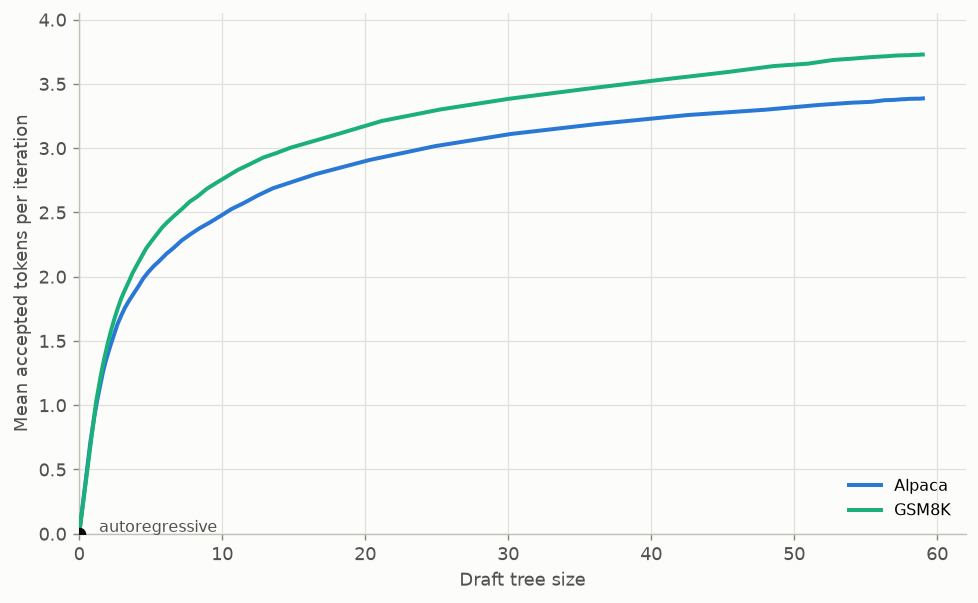
\includegraphics[width=0.8\textwidth]{Figures/draft_tree_saturation_plot.png}
\caption{Accepted tokens per decoding iteration against draft tree size after pruning.}
\label{fig:saturation}
\end{figure}

A threshold on the confidence score turns that collapse into an exchange rate. Gating at σ\textsubscript{th} = −1.5 leaves 7\% of the draft nodes on Alpaca to be verified, and those nodes still return 66.5\% of the tokens the full tree returns. Gating harder, at σ\textsubscript{th} = −1, leaves 4.5\% of the nodes and returns 59.9\% of the tokens: 22× fewer nodes verified, for 1.7× fewer tokens per iteration. GSM8K shows the same collapse, but consistently a step further along it: 69.2\% and 62.5\% of its tokens survive for 8.5\% and 5.8\% of its nodes, both above Alpaca's figures at the same gate. A tree of 59 nodes spends the great majority of its verification on the flat part of the curve, and a threshold on a score the drafting already computes is enough to keep it off.

The gap between the two datasets' acceptance rates is no coincidence. It follows from the kind of text each dataset asks the model to produce, and from how the gate responds to it. GSM8K's prompts are grade-school math word problems, and a draft model follows that kind of text more confidently than Alpaca's open-ended instructions. σ\textsubscript{th} is a fixed value on a cumulative log-probability, not a fixed tree size, so the same setting keeps whatever a draft is confident enough to justify and no more. At σ\textsubscript{th} = −1 the same threshold leaves 3.45 nodes standing on GSM8K against 2.67 on Alpaca, and those extra nodes earn their place: they return 1.96 accepted tokens against Alpaca's 1.63. The more telling question is what the gate gave up to keep them. Of the nodes it discarded at that setting, 96.9\% on Alpaca and 96.8\% on GSM8K were rejected by the target when the ungated run verified them, and loosening the gate to σ\textsubscript{th} = −1.5 puts both at 97.3\%. The gate is discarding work the target model was going to reject anyway, and it does so in nearly the same proportion on text the draft model follows easily and on text it does not. That is the second proposition holding -- the confidence score does identify which nodes are worth removing.


\subsection{Validation of the shared cost model}
\label{sec:validation}

The LP-Spec baseline is a reconstruction, for the reason Section~\ref{sec:approach} gives. Checking it therefore comes before any latency or energy result in this chapter, since the cost model that prices it produces all of them, for CAPIM and for both baselines alike. That check can only be external, and the one external reference available is what LP-Spec reports for itself: 73.4 token/s and 32.6 token/J on a 7B model~\cite{he2025lpspec}.

One quantity in the reconstruction cannot be recovered from the paper. LP-Spec's speculation length (L\textsubscript{spec}) is not a configuration value that can be set: it is produced at run-time by the Draft Token Pruner, which grows the tree node by node and stops on a combined performance and energy objective~\cite{he2025lpspec}. The paper does not specify that objective in enough detail to reproduce, so the sequence of tree sizes it would have produced cannot be regenerated. The reconstruction instead takes a fixed tree size as an input, standing for the run-average speculation length, and sweeps it over a range of settings.

Table~\ref{tab:lsweep} gives that sweep. Figure~\ref{fig:validation} places it against the two figures LP-Spec reports for itself, with the cost model driven by Alpaca traces to match the dataset LP-Spec reports those figures on. At their closest the swept sizes reproduce LP-Spec's reported energy efficiency to 0.98× and its throughput to 1.02×. An exact match was neither achieved nor expected. The reconstruction sweeps a fixed tree size in place of a run-average it cannot recover, so it yields a range rather than a single operating point. What the check asks is whether that range lands close to the reported system, and it does, to within a few percent on both of the axes LP-Spec reports.

On that basis the cost model is accepted as the instrument for the remainder of the chapter. LP-Spec accordingly enters the comparison of Section~\ref{sec:headline} not as a single quoted pair of numbers but as a modelled system swept across tree size, and CAPIM is held against the strongest point of that sweep -- a point that matches LP-Spec's published energy efficiency and exceeds its published throughput.

\begin{table}[H]
\centering
\footnotesize
\begin{tabular}{ccc}
\toprule
L\textsubscript{spec} & Throughput (token/s) & Energy efficiency (token/J) \\
\midrule
2 & 116.2 & 31.4 \\
4 & 126.9 & 31.9 \\
8 & 74.8 & 24.5 \\
12 & 58 & 21 \\
16 & 48.2 & 18.3 \\
64 & 25 & 8.9 \\
\bottomrule
\end{tabular}
\caption{The reconstructed LP-Spec baseline swept across L\textsubscript{spec}, Alpaca.}
\label{tab:lsweep}
\end{table}

\begin{figure}[H]
\centering
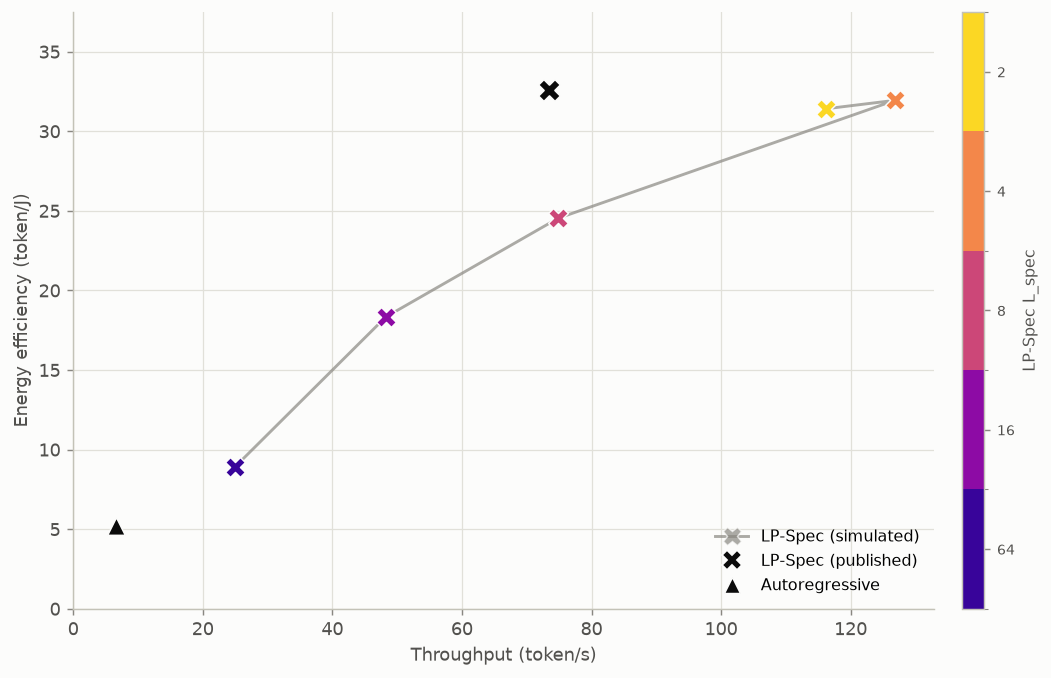
\includegraphics[width=0.8\textwidth]{Figures/cost_model_validation_plot.png}
	\caption[Reconstructed LP-Spec results on Alpaca versus its published operating point]{Reconstructed and published LP-Spec result on Alpaca, swept across L\textsubscript{spec}.}
\label{fig:validation}
\end{figure}


\subsection{Exploring the confidence–routing threshold trade-off}
\label{sec:tradeoff}

Two thresholds govern CAPIM, and neither has been given a value. Section~\ref{sec:pruning} established what a confidence gate does to the draft tree, measured against the drafting algorithm and the workload alone. The routing threshold has not been exercised at all. Both are taken up here, on the two axes upon which battery-powered device is judged, by sweeping them jointly through the cost model that Section~\ref{sec:validation} accepted.

The two thresholds are not the same kind of quantity. σ\textsubscript{th} changes what is computed: it decides how many of the 59 drafted nodes reach the verification pass, and its effect on the tree was measured in Section~\ref{sec:pruning} without reference to any hardware. μ\textsubscript{th} changes where that work is computed: every surviving tree is measured against it, and a tree smaller than the threshold has its verification pass offloaded to PIM as far as the near-bank datapath allows, while a tree larger than it has its FC kernels column-split between PIM and the NPU (Section~\ref{sec:routing}); attention stays PIM-resident in both routes. The nonlinear operations are handed to the NPU in both cases, so neither route runs on PIM alone. One threshold removes work and the other routes it.

The sweep is asked to map the exchange between the two axes and to establish what each threshold controls inside it, rather than to nominate a winner. A single objective would rank the operating points and return one optimal mode, and would discard everything else the range has to offer. A mobile device may want different operating modes in different situations. Which point is preferred can depend on the battery remaining, on the thermal headroom, and on whether a user is waiting for the output. An architecture that settles the choice at design time has answered a question the device might be better placed to answer at run-time. What the sweep is asked for is therefore the reachable region of the energy-latency plane, and the operating modes available inside it.

Table~\ref{tab:surface} gives the sweep in full, and Figure~\ref{fig:surface_alpaca} draws the Alpaca half of it. Each setting of the confidence gate traces its own curve through the plane, and μ\textsubscript{th} is travel along that curve, from the fast, high-power corner at μ\textsubscript{th} = 1 to the slow, low-power one at μ\textsubscript{th} = 64. The curves are long enough to be worth having. Holding σ\textsubscript{th} at −1 and moving μ\textsubscript{th} alone carries the design from 153 token/s at 46.2 token/J to 138.8 token/s at 63.8 token/J, which buys 38\% more energy efficiency for 9\% less throughput. The same movement is present at every gate. This is the exchange the architecture offers, and μ\textsubscript{th} is the control that walks along it.


\begin{table}[H]
\centering
\footnotesize
\setlength{\tabcolsep}{4.5pt}
\begin{tabular}{lccccccc}
\toprule
 & \multicolumn{7}{c}{μ\textsubscript{th}} \\
\cmidrule(lr){2-8}
σ\textsubscript{th} & 1 & 2 & 4 & 8 & 12 & 16 & 64 \\
\midrule
\multicolumn{8}{l}{\emph{Alpaca}} \\
−0.5 & 151.0 / 43.9 & 144.6 / 51.7 & 141.7 / 56.5 & 138.4 / 60.6 & 138.4 / 60.6 & 138.4 / 60.6 & 138.4 / 60.6 \\
−1.0 & 153.0 / 46.2 & 149.6 / 50.3 & 146.2 / 55.3 & 139.1 / 63.6 & 138.9 / 63.8 & 138.8 / 63.8 & 138.8 / 63.8 \\
−1.5 & 142.1 / 45.8 & 140.9 / 47.3 & 138.8 / 50.4 & 128.6 / 61.8 & 126.4 / 64.3 & 126.2 / 64.4 & 126.2 / 64.4 \\
−2.0 & 123.6 / 42.9 & 123.3 / 43.3 & 122.6 / 44.4 & 114.4 / 53.0 & 107.7 / 60.7 & 106.4 / 62.1 & 106.3 / 62.2 \\
−2.5 & 103.2 / 38.4 & 103.1 / 38.5 & 103.0 / 38.7 & 99.8 / 41.8 & 91.6 / 49.6 & 86.1 / 55.8 & 84.2 / 58.0 \\
\midrule
\multicolumn{8}{l}{\emph{GSM8K}} \\
−0.5 & 160.3 / 47.7 & 155.5 / 53.6 & 152.1 / 58.8 & 146.1 / 65.9 & 146.1 / 65.9 & 146.1 / 65.9 & 146.1 / 65.9 \\
−1.0 & 155.5 / 48.8 & 153.6 / 51.2 & 150.6 / 55.4 & 140.1 / 67.5 & 139.8 / 67.8 & 139.8 / 67.8 & 139.8 / 67.8 \\
−1.5 & 140.1 / 47.3 & 139.7 / 47.8 & 138.4 / 49.7 & 126.1 / 63.5 & 123.3 / 67.0 & 123.1 / 67.2 & 123.1 / 67.2 \\
−2 & 120.1 / 43.2 & 120.0 / 43.3 & 119.7 / 43.8 & 112.2 / 51.4 & 104.1 / 60.8 & 102.3 / 63.0 & 101.9 / 63.4 \\
−2.5 & 102.6 / 39.0 & 102.6 / 39.0 & 102.5 / 39.1 & 100.4 / 41.1 & 92.0 / 48.7 & 85.3 / 56.1 & 82.6 / 59.3 \\
\bottomrule
\end{tabular}
\caption{The joint threshold sweep, as throughput (token/s) / energy efficiency (token/J).}
\label{tab:surface}
\end{table}

\begin{figure}[H]
\centering
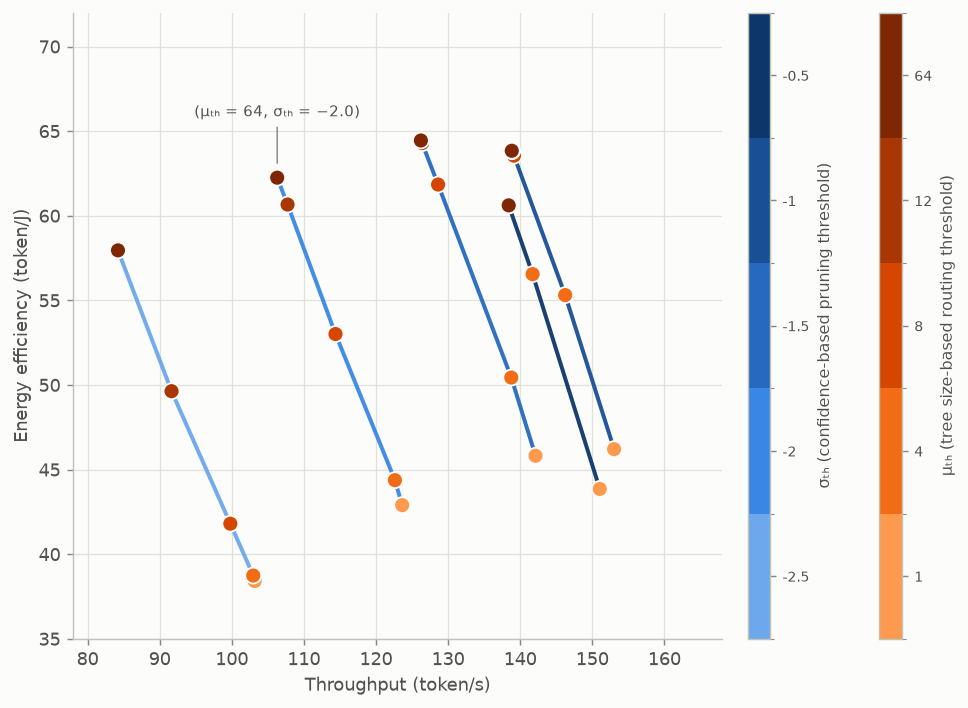
\includegraphics[width=0.85\textwidth]{Figures/threshold_tradeoff_alpaca_plot.png}
\caption{The (σ\textsubscript{th}, μ\textsubscript{th}) sweep on Alpaca. Line colour encodes σ\textsubscript{th}, dot fill μ\textsubscript{th}.}
\label{fig:surface_alpaca}
\end{figure}

The two thresholds are connected, since the largest tree a gate ever produces sets a ceiling on what the routing threshold can still act on. Once μ\textsubscript{th} passes that ceiling, no tree the gate produces is large enough to cross it, so every higher setting routes every tree the same way and returns the same numbers. Table~\ref{tab:trees} gives the tree that survives each setting of σ\textsubscript{th}, and its largest-tree column locates that ceiling in each row of Table~\ref{tab:surface}. On Alpaca, σ\textsubscript{th} = −0.5 produced no tree larger than 6 nodes, and its μ\textsubscript{th} = 8, 12, 16 and 64 entries are accordingly identical; at σ\textsubscript{th} = −1 the largest tree observed is 12 and the entries become identical from μ\textsubscript{th} = 16; at σ\textsubscript{th} = −2.5 the largest is 27 and the row is still moving at 64. The correspondence holds in all ten rows across both datasets. Where each row's ceiling falls is a property of these traces and not a guarantee, since a prompt that drafted a larger tree at a tight gate would push it out.

\begin{table}[H]
\centering
\footnotesize
\begin{tabular}{lcccccc}
\toprule
 & \multicolumn{3}{c}{Alpaca} & \multicolumn{3}{c}{GSM8K} \\
\cmidrule(lr){2-4}\cmidrule(lr){5-7}
σ\textsubscript{th} & median & mean & largest & median & mean & largest \\
\midrule
−0.5 & 1 & 1.59 & 6 & 2 & 2.18 & 6 \\
−1 & 2 & 2.63 & 12 & 3 & 3.39 & 11 \\
−1.5 & 4 & 4.05 & 14 & 5 & 5.02 & 15 \\
−2 & 6 & 6.08 & 18 & 7 & 7.16 & 20 \\
−2.5 & 9 & 9.11 & 27 & 10 & 10.32 & 29 \\
\bottomrule
\end{tabular}
\caption{The draft tree size in nodes after confidence-based pruning}
\label{tab:trees}
\end{table}

Figure~\ref{fig:surface_gsm8k} draws the same sweep on GSM8K, and its surface sits up and to the right of Alpaca's throughout: 160.3 token/s at its fastest against 153, and 67.8 token/J at its most efficient against 64.4. This is the expected result. Section~\ref{sec:pruning} found GSM8K's more confident draft keeping a larger share of its tree at every gate, and that advantage carries through to every point on this surface. What the two surfaces do not agree on is where the gate itself should sit. Alpaca's fastest point belongs to σ\textsubscript{th} = −1 and GSM8K's to the tighter σ\textsubscript{th} = −0.5. The gate is an absolute threshold rather than a fixed tree size, so the same number does not select the same tree on a more confident workload.

\begin{figure}[H]
\centering
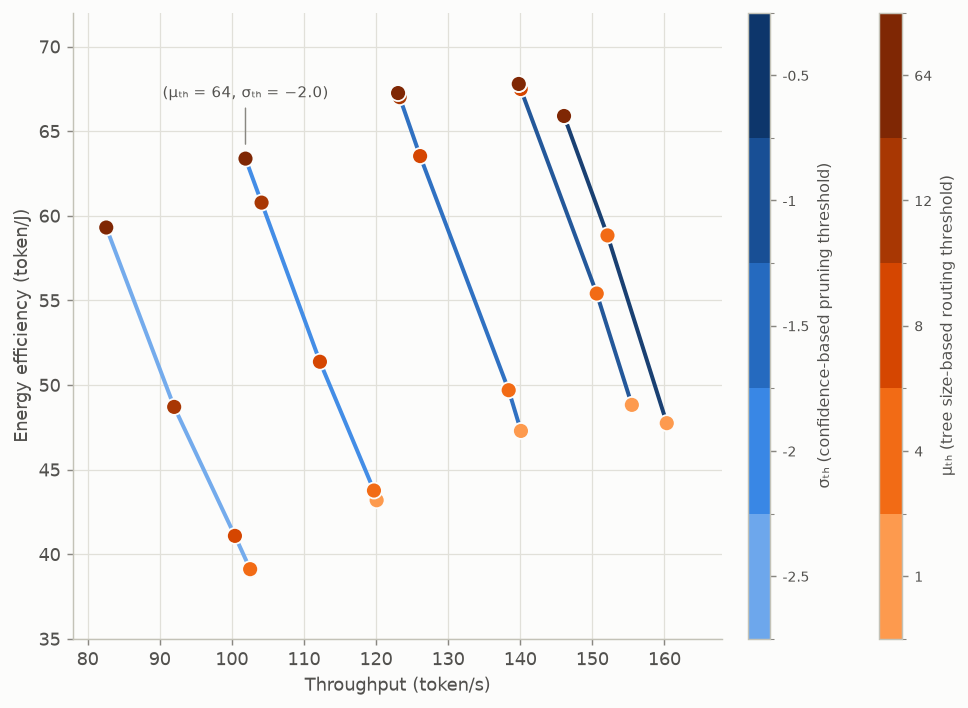
\includegraphics[width=0.85\textwidth]{Figures/threshold_tradeoff_gsm8k_plot.png}
\caption{The (σ\textsubscript{th}, μ\textsubscript{th}) sweep on GSM8K. Line colour encodes σ\textsubscript{th}, dot fill μ\textsubscript{th}.}
\label{fig:surface_gsm8k}
\end{figure}

The sweep can rule some gates out, but it cannot pick one. σ\textsubscript{th} = −2 improves on σ\textsubscript{th} = −2.5 on both throughput and energy efficiency, at all seven settings of μ\textsubscript{th} and on both datasets, and σ\textsubscript{th} = −1.5 improves on −2 the same way. The two loosest gates are therefore excluded, without any judgement about how energy trades against latency. No such comparison exists among the three tightest gates, since each wins on one axis somewhere in the range, so ranking them would need a preference the sweep is not entitled to supply. That leaves σ\textsubscript{th} between −1.5 and −0.5, a band in which the surviving tree averages 1.6 to 5 nodes of the 59 drafted (Table~\ref{tab:trees}). Neither threshold is fixed there, and both stay run-time controls.

\subsection{Headline results}\label{sec:headline}

Section~\ref{sec:tradeoff} swept σ\textsubscript{th} and μ\textsubscript{th} jointly and did not resolve either to a single value. σ\textsubscript{th} is bounded to between −1.5 and −0.5 by pairwise dominance and left there; μ\textsubscript{th} was shown to move the design along a throughput--energy exchange at whichever gate σ\textsubscript{th} is set to, from a fast, high-power corner at μ\textsubscript{th} = 1 to a slow, low-power corner at μ\textsubscript{th} = 64. Both remain run-time controls, not values compiled into the design. What this section adds is a comparison: fixing σ\textsubscript{th} to a single value and μ\textsubscript{th} to two, so that CAPIM can be placed against LP-Spec and against standard autoregressive decoding at concrete, reproducible points rather than as a region.

Two settings are carried forward, one from each corner of the throughput--energy exchange, both holding σ\textsubscript{th} at −1: \emph{Standard} (μ\textsubscript{th} = 1) and \emph{Low-power} (μ\textsubscript{th} = 64). At μ\textsubscript{th} = 1 that gate dominates both of its neighbours in the −1.5-to−0.5 range outright (Table~\ref{tab:surface}: 153 token/s / 46.2 token/J beats −0.5's 151/43.9 and −1.5's 142.1/45.8 on both axes at once). At μ\textsubscript{th} = 64 it still dominates −0.5 outright, and against −1.5 it trades under one percent of energy efficiency for ten percent more throughput (138.8/63.8 against 126.2/64.4) -- not strict dominance, but decisive enough to make the same choice at both ends.

Figure~\ref{fig:headline} places both CAPIM points against LP-Spec and against autoregressive decoding. GSM8K is left out: LP-Spec has no published result on that dataset, and comparing CAPIM's GSM8K numbers against a baseline that was never evaluated there would not be a fair reading. Both CAPIM points sit above and to the right of both LP-Spec references on both axes at once. Autoregressive decoding -- which runs entirely on the NPU with no speculative decoding applied -- sits far enough below either that it only anchors the scale.

\begin{figure}[H]
\centering
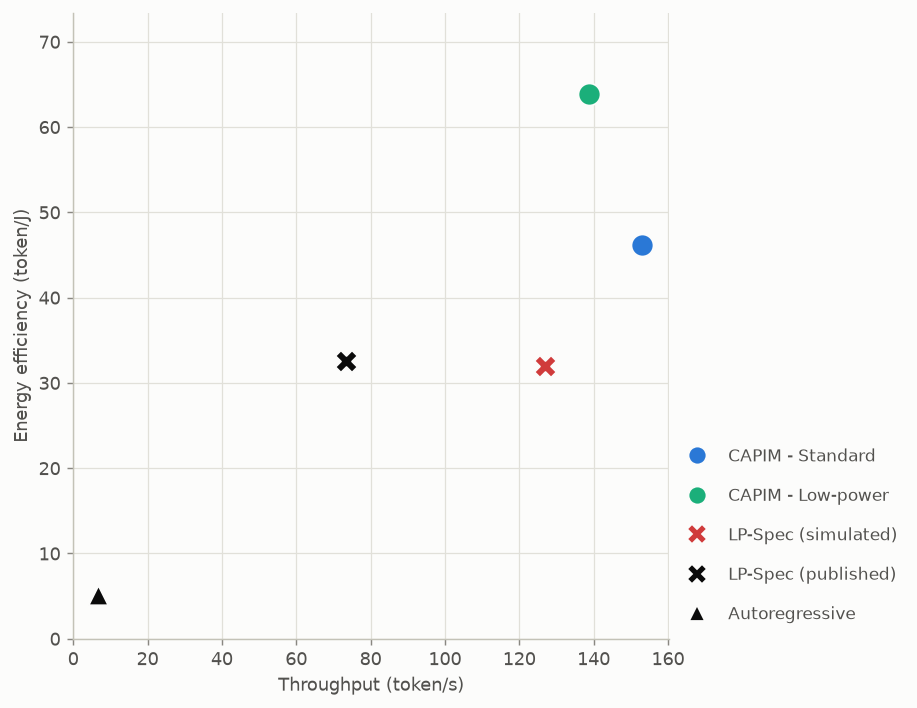
\includegraphics[width=0.72\textwidth]{Figures/headline_comparison_alpaca_plot.png}
\caption{CAPIM against LP-Spec and autoregressive decoding, Alpaca.}
\label{fig:headline}
\end{figure}

\begin{table}[H]
\centering
\footnotesize
\begin{tabular}{lccc}
\toprule
 & Throughput (token/s) & Energy efficiency (token/J) & EDP (s\textperiodcentered mJ) \\
\midrule
CAPIM -- Standard & 153 & 46.2 & 0.141 \\
CAPIM -- Low-power & 138.8 & 63.8 & 0.113 \\
LP-Spec (simulated, best) & 126.9 & 31.9 & 0.247 \\
LP-Spec (published) & 73.4 & 32.6 & 0.418 \\
Autoregressive & 6.5 & 5.2 & 29.5 \\
\bottomrule
\end{tabular}
\caption{The values underlying Figure~\ref{fig:headline}, including energy-delay product (EDP), Alpaca.}
\label{tab:headline_values}
\end{table}

Table~\ref{tab:headline_ratio} restates the same comparison as ratios. Against LP-Spec's best simulated configuration, Standard reaches 1.21× the throughput and 1.45× the energy efficiency, and Low-power reaches 1.09× and 2.00×. Against LP-Spec's own published pair the margin widens further, to 2.08×/1.42× and 1.89×/1.96×. The result worth pointing out is Low-power's throughput. Low-power is the setting tuned to trade throughput away for energy efficiency, yet against LP-Spec's best simulated configuration it doubles the energy efficiency while still running faster.

\begin{table}[H]
\centering
\footnotesize
\begin{tabular}{lcccc}
\toprule
 & \multicolumn{4}{c}{CAPIM} \\
\cmidrule(lr){2-5}
 & \multicolumn{2}{c}{Standard} & \multicolumn{2}{c}{Low-power} \\
\cmidrule(lr){2-3}\cmidrule(lr){4-5}
Baseline & token/s & token/J & token/s & token/J \\
\midrule
LP-Spec (simulated, best) & 1.21×  & 1.45× & 1.09×  & 2.00×  \\
LP-Spec (published)       & 2.08×  & 1.42× & 1.89×  & 1.96×  \\
Autoregressive            & 23.38× & 8.92× & 21.21× & 12.33× \\
\bottomrule
\end{tabular}
\caption{CAPIM's two operating points as ratios to each baseline, Alpaca.}
\label{tab:headline_ratio}
\end{table}

The targets set for this project in Section~\ref{subsec:objectives} are a 20--30\% improvement in energy efficiency and 1.5×--2× in throughput over LP-Spec. The energy target is met and then exceeded. Even Standard, the faster of the two settings, is 45\% more energy-efficient than LP-Spec's best simulated configuration, and Low-power reaches 2.00×. The throughput target is not met against LP-Spec's best simulated configuration, where Standard reaches only 1.21× and Low-power 1.09×, though it is met against LP-Spec's own published figure, where Standard reaches 2.08× and Low-power 1.89×. The shortfall against LP-Spec's best configuration is structural. Medusa fires every one of its heads in a single parallel pass, proposing an entire candidate tree in one shot. EAGLE-2's draft model instead runs autoregressively, reading back its own hidden state one step at a time to grow the tree, and that sequential cost is one Medusa never pays. CAPIM's higher acceptance rate and smaller, better-targeted tree earn back most of that cost against LP-Spec's fastest configuration, but not all of it.

The two settings are chosen points on that exchange, not the only ones available. μ\textsubscript{th} is a run-time control rather than a value fixed at design time, and Section~\ref{sec:tradeoff} swept the range between Standard and Low-power, so a device can move between them according to its own battery and thermal state. That run-time controllability is itself part of this project's contribution, and it is easy to lose sight of when two points stand in for the whole range.

% ---------- Conclusion ----------
\newpage
\section{Conclusion}

This work proposed and evaluated CAPIM, a mobile LLM inference architecture that pairs LPDDR5-PIM with a mobile NPU and runs EAGLE-2 speculative decoding natively. A hardware controller drives the decode loop from end to end. It grows the draft tree only while the confidence accumulated along a branch stays above a threshold σ\textsubscript{th}, and it routes verification of the surviving tree between the PIM and the NPU by the tree's size, against a routing threshold μ\textsubscript{th}. The design was assessed against LP-Spec, the state-of-the-art mobile PIM baseline, and against plain autoregressive decoding, all three priced on one shared analytical cost model so the comparison turns on the architecture alone.

The first phase of the work studied EAGLE-2's draft trees on their own, before any hardware was committed to a pruner, to find whether a confidence-based stopping rule was available at all. EAGLE-2 accumulates a confidence score along each branch and uses it to rank candidates, expanding and verifying a fixed number of them, so the tree comes out the same size at every decoding iteration whatever the context. A gate needs that score in absolute terms, since it must judge one branch on its own. Section~\ref{sec:pruning} shows the accepted tokens concentrating in the first few nodes of the tree -- the first three on Alpaca yield 0.59 accepted tokens each, against 0.033 for the 56 that follow. A threshold on the accumulated score separates the two. Gating at σ\textsubscript{th} = −1 leaves 4.5\% of the drafted nodes to be verified and still returns 59.9\% of the tokens the full tree returns, and 96.9\% of what it discards would have been rejected by the target in any case. Whether that exchange is a good one depends on what verification costs to run, which the trees on their own cannot say. What they do say is that the score tracks acceptance closely enough for a threshold to act on, and that was reason enough to carry the gate into the next phase and price it on the cost model.

The second phase evaluated the full architecture, pricing both of its thresholds against the LP-Spec baseline and against plain autoregressive decoding on the shared cost model. σ\textsubscript{th} decides how much of the draft tree reaches verification, and μ\textsubscript{th} decides where that verification runs. Sweeping the two jointly did not return a single best design, and was not asked to. What it returned was a range. At whichever gate σ\textsubscript{th} is set to, μ\textsubscript{th} carries the design from a fast, high-power corner, where verification splits its FC kernels across the NPU, to a slow, low-power one where it stays in the memory with no weights crossing the off-chip interface. A battery-constrained device has no fixed exchange rate between latency and energy, since the right balance depends on its live battery and thermal state, so that range is worth more than any point inside it. LP-Spec's Data Allocation Unit, by contrast, fixes the placement internally to a latency objective and splits the work unconditionally, paying to move a share of the weights off-chip on every pass. What this phase established is that the same decision can be re-cast as a battery-aware policy the device sets at run time.

Measured against LP-Spec, CAPIM exceeds this project's energy target and partly meets its throughput target. The two operating points reported in Section~\ref{sec:headline} bracket the range μ\textsubscript{th} opens up. Standard, the faster of them, reaches 1.45× the energy efficiency of LP-Spec's best simulated configuration while also running 1.21× faster, and Low-power reaches 2.00× the energy efficiency at 1.09× the throughput; against LP-Spec's published pair both are faster still, at 2.08× and 1.89×. The 20--30\% energy target is therefore cleared with margin at both settings. The 1.5×--2× throughput target is met against the published figure, but not against the fastest simulated configuration, where the margin narrows to 1.21× and 1.09×. That shortfall is structural, and Section~\ref{sec:headline} traces it to EAGLE-2's draft model, which grows its tree one step at a time where Medusa proposes a whole tree in a single parallel pass.

The two run-time controls the architecture exposes are not left equally well understood, and the gap between them is the clearest opening for further work. μ\textsubscript{th} is ready to deploy: it moves the design monotonically along the energy--throughput exchange, its two ends have a clear meaning, and a device can turn it against its own battery and thermal state without further characterization. σ\textsubscript{th} is not in that state. This work fixed it by sweeping both datasets and taking the value that performed best, which is an experimental result rather than a rule a practitioner can apply to a new model or workload without repeating the sweep. Future work should replace that calibration with a principled way to set the gate, such as adapting σ\textsubscript{th} online as decoding proceeds based on a moving average of recent verification outcomes.

Several further directions follow from the design as it stands. EAGLE-3~\cite{li2025eagle3} is a newer speculative decoding method in the same family, and it shapes its draft tree from the same confidence score. Adapting CAPIM to run on it is a natural next step, and one this project could not take without training a draft model of its own, since no 7B backbone has both a published EAGLE-3 draft model and the Medusa heads the LP-Spec baseline requires for a fair comparison. A second direction is longer-context workloads, where pinning attention to the memory should pay off more as the key-value cache grows, a regime the two short-context datasets used here never reach.

The three questions the project set out to test are answered, and together their answers are what CAPIM contributes. A mobile PIM architecture can adopt EAGLE-2 speculative decoding natively and outperform the state of the art, reaching between 1.45× and 2.00× the energy efficiency of LP-Spec's best simulated configuration while running faster than it at both settings. EAGLE-2's confidence scores, accumulated along a branch, serve as a live pruning criterion that a gate can act on directly. The size of the tree that gate leaves standing then routes verification between the PIM and the NPU, leaving a mobile device to set the balance between energy and latency for itself rather than inheriting it fixed from the hardware.

% ---------- References ----------
\newpage
\addcontentsline{toc}{section}{References}
\bibliographystyle{IEEEtran}
\bibliography{references} 

\end{document}
